\chapter{Trajectory planning}

When doing control theory, the goal is often (and also in the present case) to have the system follow a predefined behaviour. In the L-PBF system that means for the scanner movement to follow a predefined scan pattern. The scanner movement has two fundamentally different modes of operation:
\begin{itemize}
    \item When the laser is on and thus melting the metal powder it is very important to have precise control of the velocity and position. The trajectories that the laser travels along while it's turned on, will be called \textit{scan} trajectories in this section. The scan trajectories are strictly determined by the geometry of the object that is to be build. As the material-energy interaction within L-PBF defines not only the geometry but also the material properties it is critical to maintain a well-defined energy density across each scan trajectory. This can be achieved by keeping constant laser source power, and constant velocity.
    \item While the laser is off, it can be decided more freely how the scanner should move (but it needs to get to the next scan path in some way). However, the movement in this scenario influences the performance during the on-phases through the inertia of the mirrors. The trajectories travelled while the laser is off will be called \textit{travel} trajectories.
\end{itemize}

The idea is then to optimise the travel trajectories to give the scanner the best possible chance to follow the scan trajectories perfectly. The key element is to plan the travel trajectory so that the scanner already has the correct velocity when the scan trajectory begins, also called sky riding. This is done to solve the following problem: if the scanner is at standstill when beginning the scan trajectory the laser will move slow on the first part until it has accelerated to the correct speed. During this slow part the energy density in the melt pool will be too high, resulting in uneven and unpredictable results.

In the current system design all the scan and travel trajectories are straight line segments with constant velocity. This section is about finding better options for the travel trajectories, so as to keep the process parameters, especially the energy density stable during the scan paths. All the way through the planning it is assumed that the travel trajectories are immediately preceded and followed by scan trajectories and that the end position of the preceding scan trajectory is different from the start position of the following scan trajectory. There is a use case for trajectory planning where these positions are the same, eg. when doing corners in the contour. In Section \ref{sec:trajectory-discussion} it is discussed how the methods could be adapted for this.

\section{Choosing the best trajectory planning method}

The scanner system has good conditions for trajectory planning as there are no areas in the image plane that must be avoided. The only limits are a speed limit of the scanner and the outer bounds of the image plane. Also the movement of the two mirrors and more specifically the movement of the x-position and y-position of the laser in the image plane can be reasonably assumed to be independent as discussed in Section \ref{sec:kinematic-model}. While it was found in section \ref{sec:f-theta-dev-angle} that this assumption is only an approximation, the approximation proves to be accurate enough, especially combined with calibration, to be usable for the trajectory planning.

Three different methods were considered for the planning of the trajectories: Cubic Polynomial, Quintic Polynomial and Linear Segments with Parabolic Blends (LSPB) \cite[chapter 5.5.1]{robot-control}. LSPB seemed the obvious choice, because the geometries that the printer is build to produce consist of linear segments with constant velocity. But that strategy is made for starting and ending at standstill and it would be preferable to do without stopping and start for every line segment as common geometries contain thousands of line segments.

Between the cubic polynomial and the quintic polynomial the difference is whether or not to have control of acceleration also in addition to the velocity. For the L-PBF it is important to have control of the acceleration because it is not only the instantaneous velocity at the beginning of the scan path that is of interest. The velocity needs to be constant through out the scan trajectory which means an acceleration of zero is required. A non-zero acceleration at the beginning of the scan path would mean that even though the velocity is correct at that particular time, it is about to change, rather than being constant. As a result, the quintic polynomial method seems best fit for purpose.

\section{Calculating the quintic polynomial trajectories} \label{sec:calc-quintic-poly}

The trajectories for the movement in x- and y-direction are calculated in the same way but independently. So for readability this section uses \textit{positions} (in the plural) to mean \textit{x- and y-positions}, and likewise for velocities and accelerations.

The quintic polynomial method works in the following way:
\begin{enumerate}
    \item A starting time and an end time for the trajectory are set.
    \item Boundary conditions for positions, velocities and accelerations are set. That is, the values for positions, velocities and accelerations in the start and end of the trajectory are chosen to match the previous and following scan trajectories.
    \item The positions are assumed to follow quintic (5th order) polynomial functions of time. The six coefficients of both of these polynomials are then derived (and uniquely determined) from the two pairs of six equations that follow from the boundary conditions.
\end{enumerate}

Without loss of generality, the starting time can be set to $t_0 = 0$. The choice of end-time,  $t_1$, can be optimised for different properties. For the purpose of this thesis, a \textit{good enough} way to determine it is by calculating it from a chosen absolute average velocity, $\bar{v}_{travel}$, of the travel trajectory and the direct distance, $\Delta s_{travel}$, from the starting point to the end point in the image plane. This is expressed in Equation \ref{eq:quintic-t1} where $\Delta s_{travel}$ is calculated from the start and end coordinates with Pythagoras theorem.
\begin{align}
    t_1 = \frac{\Delta s_{travel}}{\bar{v}_{travel}} \label{eq:quintic-t1}
\end{align}

The boundary conditions, that the trajectory should fulfil at times $t_0$ and $t_1$ are determined by the previous and following scan paths. Obviously the start positions of the travel path must be the same as the end positions of the previous scan path, and like wise the end positions of the travel path must be equal to the start positions of the next scan path. The velocities and accelerations are determined in exactly the same way. Notably the accelerations in both beginning and end are zero, since the scan paths have constant velocity.

Having set the boundary conditions at the beginning and end-time of the trajectories means that the polynomials can now be determined. The task is to find the $\beta$ coefficients in Equation \ref{eq:cp1} and \ref{eq:cp2} where $s_x$ and $s_y$ are the displacement of the melt pool relative to the image plane (the laser is off during these trajectories, so "melt pool" is to be taken as "where the melt pool would be if the laser was turned on").

\begin{align}
    s_x(t) = \beta_{x0} + \beta_{x1}*t + \beta_{x2}*t^2 + \beta_{x3}*t^3 + \beta_{x4}*t^4 + \beta_{x5}*t^5 \label{eq:cp1}\\
    s_y(t) = \beta_{y0} + \beta_{y1}*t + \beta_{y2}*t^2 + \beta_{y3}*t^3 + \beta_{y4}*t^4 + \beta_{y5}*t^5 \label{eq:cp2}
\end{align}

Firstly, substituting position and time for beginning and end gives two equations for each polynomial. The expressions for the velocities are produced by taking the derivative with respect to time. Substituting the velocities and time for beginning and end in these produces two additional equations for each polynomial. Lastly, taking the second derivative with respect to time gives expressions for the accelerations and again by inserting the boundary conditions, the last two equations that are needed are found. The set of equations for the movement of each variable are identical except for boundary condition constants. Both sets can be expressed in matrix form as in Equation \ref{eq:quintic-beta}.

\begin{align}
    \begin{bmatrix}
        1  & t_0  & t_0^2    & t_0^3    & t_0^4    & t_0^5 \\
        0  & 1   & 2t_0    & 3t_0^2  & 4t_0^3  & 5t_0^4 \\
        0  & 0   & 2       & 6t_0    & 12t_0^2 & 20t_0^3 \\
        1  & t_1  & t_1^2    & t_1^3    & t_1^4    & t_1^5 \\
        0  & 1   & 2t_1    & 3t_1^2  & 4t_1^3  & 5t_1^4 \\
        0  & 0   & 2       & 6t_1    & 12t_1^2 & 20t_1^3
    \end{bmatrix}
    \begin{bmatrix}
        \beta_{0} \\
        \beta_{1} \\
        \beta_{2} \\
        \beta_{3} \\
        \beta_{4} \\
        \beta_{5}
    \end{bmatrix}
    =
    \begin{bmatrix}
        s_{0} \\
        v_{0} \\
        a_{0} \\
        s_{1} \\
        v_{1} \\
        a_{1} \\        
    \end{bmatrix}
    \label{eq:quintic-beta}
\end{align}

The equations simplify significantly for $t_0 = 0$, $a_{0} = a_{1} = 0$ giving the solutions in Equations \ref{eq:beta_x0} - \ref{eq:beta_x5}. Again these equations are identical for x and y movement, except for the boundary condition constants, giving a distinct set of $\beta$ coefficients and thus trajectory for each variable.

\begin{align}
    \beta_{0} &= s_{0} \label{eq:beta_x0} \\
    \beta_{1} &= v_{0} \\
    \beta_{2} &= 0 \\
    \beta_{3} &= -\frac{2\,{\left(5\,s_{\textrm{0}} -5\,s_{\textrm{1}} +3\,t_1 \,v_{\textrm{0}} +2\,t_1 \,v_{\textrm{1}} \right)}}{{t_1 }^3 } \\
    \beta_{4} &= \frac{15\,s_{\textrm{0}} -15\,s_{\textrm{1}} +8\,t_1 \,v_{\textrm{0}} +7\,t_1 \,v_{\textrm{1}} }{{t_1 }^4 } \\
    \beta_{5} &= -\frac{3\,{\left(2\,s_{\textrm{0}} -2\,s_{\textrm{1}} +t_1 \,v_{\textrm{0}} +t_1 \,v_{\textrm{1}} \right)}}{{t_1 }^5 } \label{eq:beta_x5}
\end{align}

For $v_{0}=v_{1}$, the equations simplify (quite beautifully) even further. This condition is true for almost all cases. The only exceptions are travel trajectories with hatching lines on one end and contour lines on the other. In this case the boundary condition on velocity can be different for start and end (hatching and contour can use different scan speeds), but otherwise the velocity in the beginning and end of a travel trajectory will be the same. With the coefficients of the polynomials determined, everything is there for a complete description of the desired movement of the laser in the image plane. This trajectory is guaranteed to satisfy the boundary conditions set in the beginning. An example of a travel trajectory can be seen on Figures \ref{fig:5-traj-pos} and \ref{fig:5-traj-vel-acc}

\begin{figure}
    \centering
    \begin{subfigure}{0.72\textwidth}  
        \centering 
        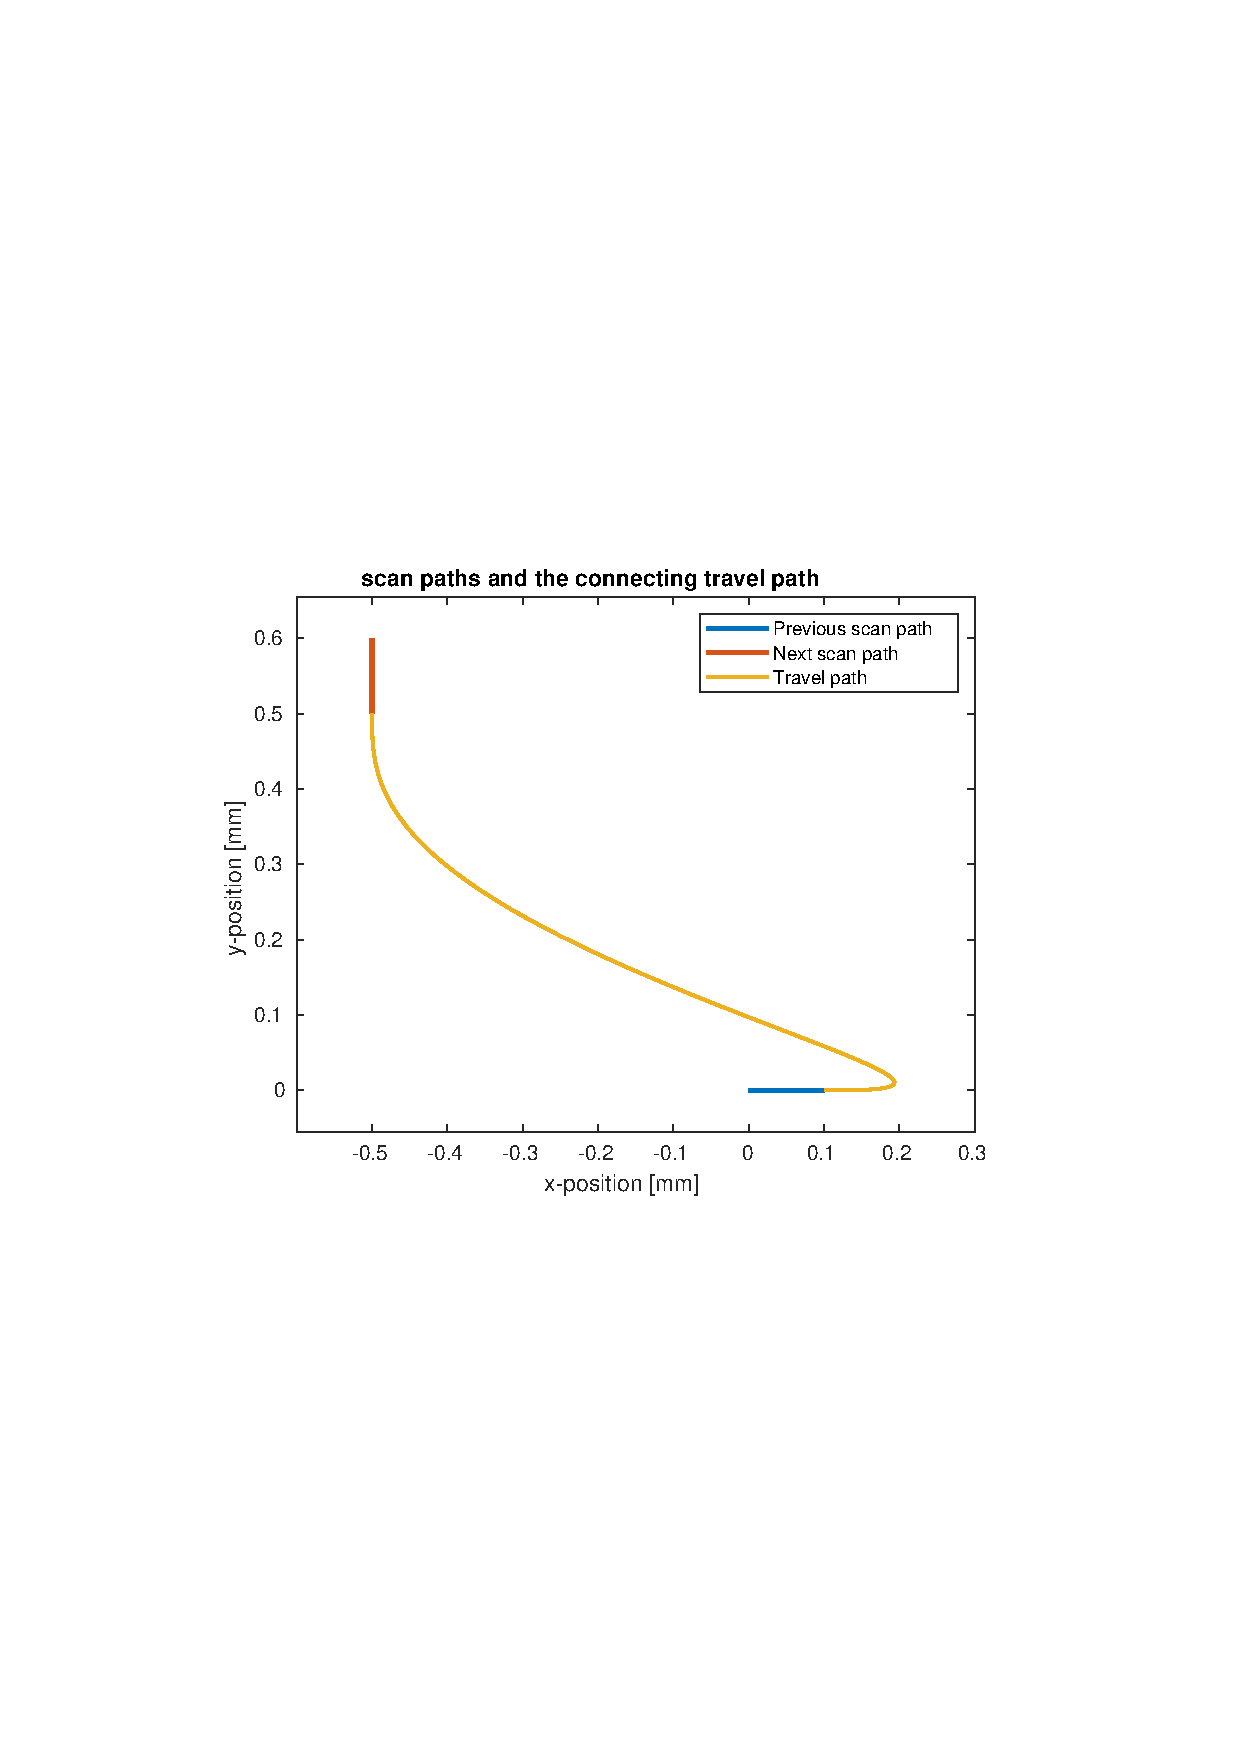
\includegraphics[clip, trim=3.5cm 9cm 4cm 9cm, width=\textwidth]{Pictures/scan-travel-path.pdf}
        \caption{An example of two scan paths and a travel path that brings the laser from one to the other}    
        \label{fig:5-traj-pos-pos}
    \end{subfigure}
    \vskip\baselineskip
    \begin{subfigure}{0.72\textwidth}   
        \centering 
        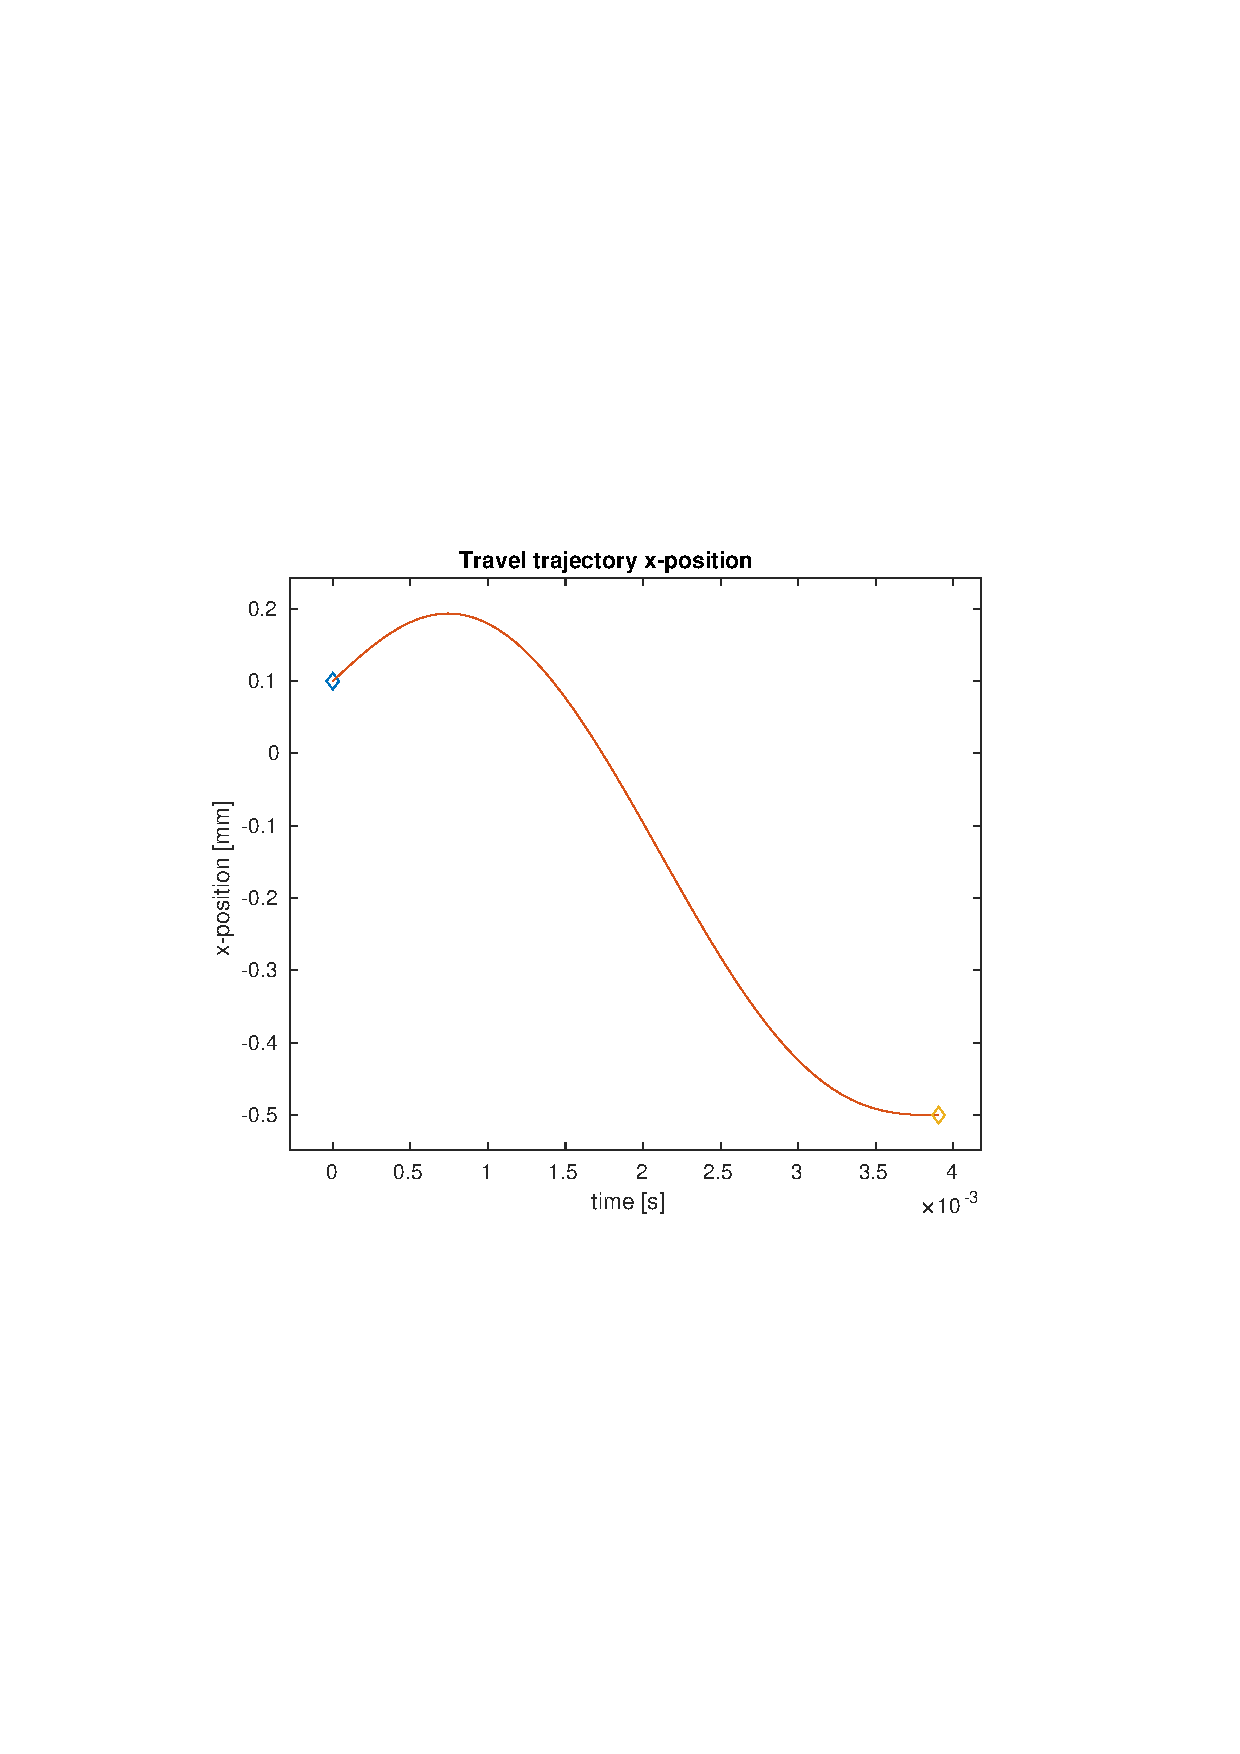
\includegraphics[clip, trim=3.5cm 9cm 4cm 9cm, width=\textwidth]{Pictures/5-traj-pos.pdf}
        \caption{The x-position plotted over time, together with the end x-position of the previous scan path, and the start x-position of the next. This figure shows that the travel path complies with the boundary conditions on position.}
        \label{fig:5-traj-pos-t}
    \end{subfigure}
    \caption{}
    \label{fig:5-traj-pos}
\end{figure}

\begin{figure}
    \centering
    \begin{subfigure}{0.72\textwidth}   
        \centering 
        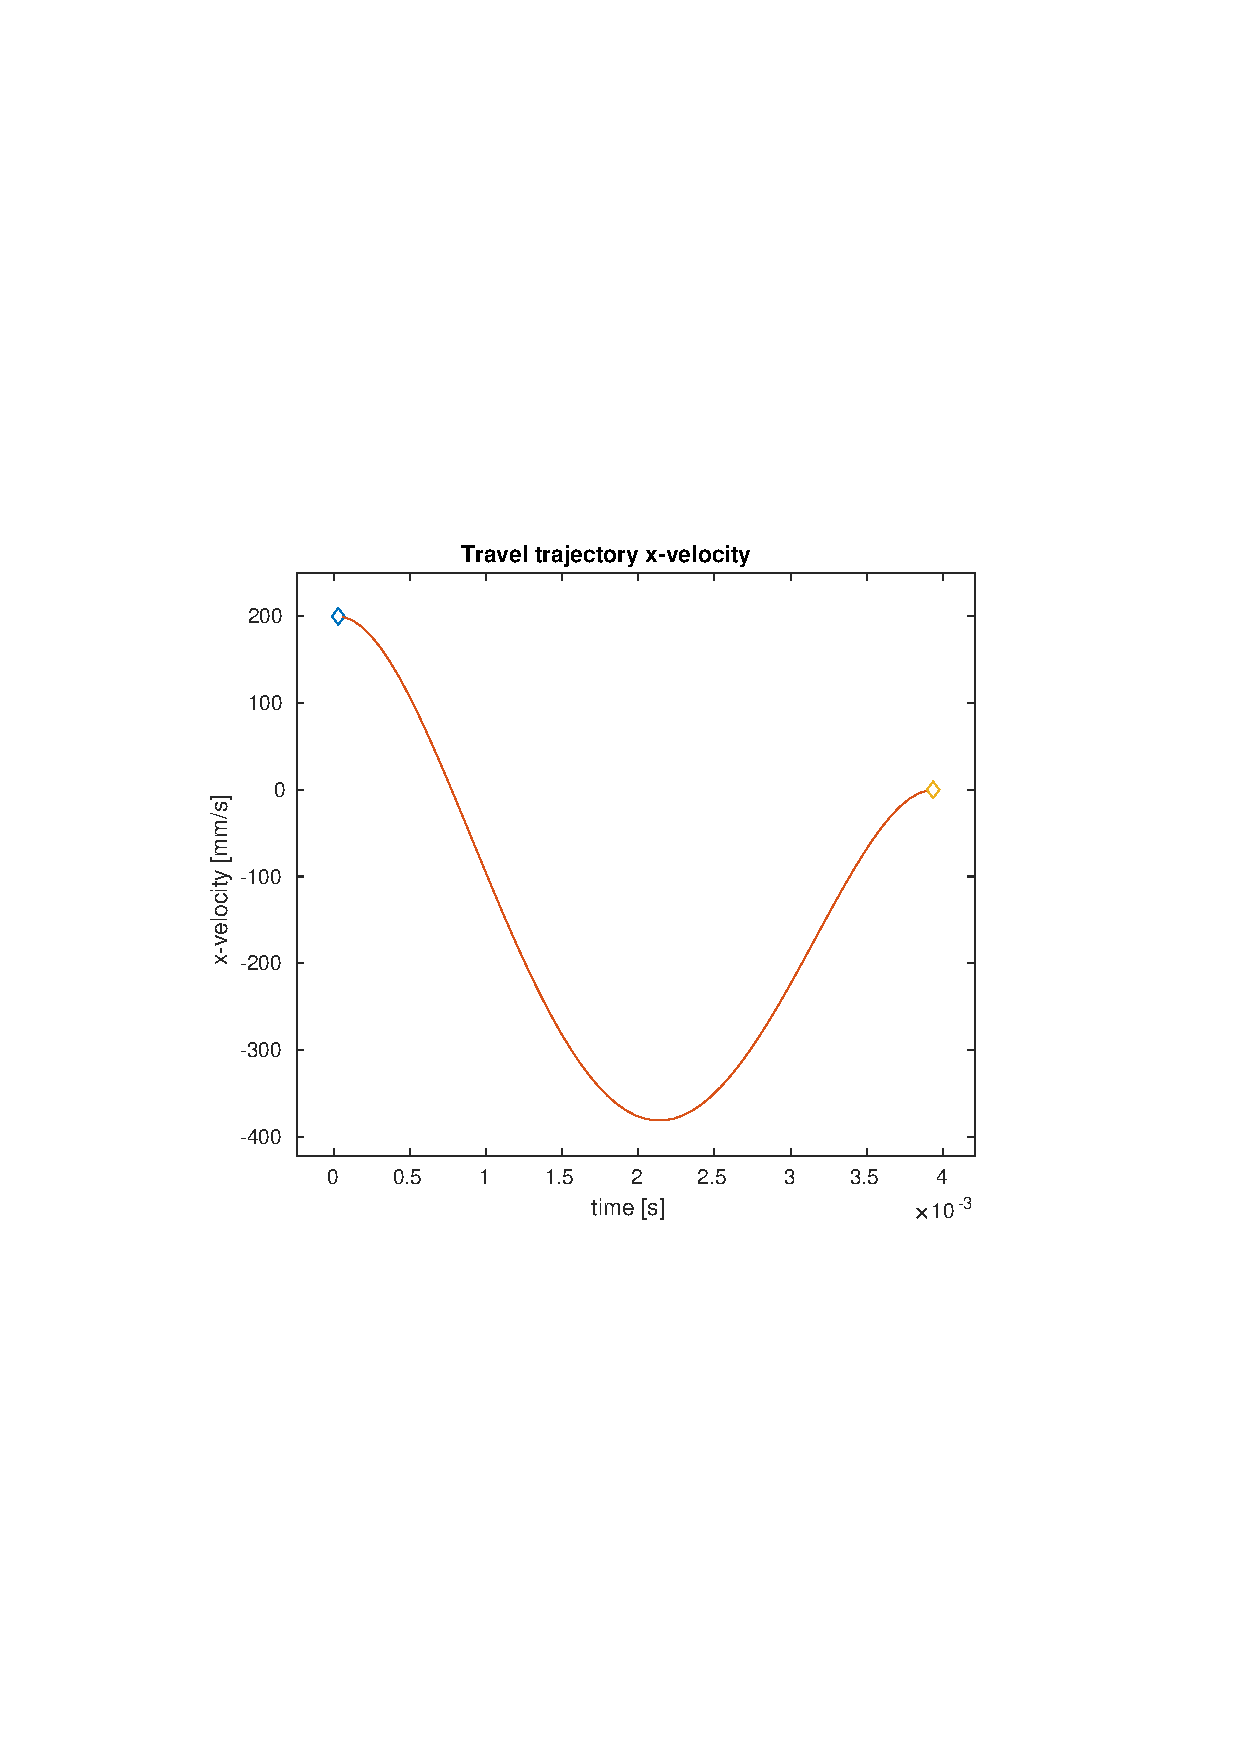
\includegraphics[clip, trim=3.5cm 9cm 4cm 9cm, width=\textwidth]{Pictures/5-traj-vel.pdf}
        \caption{The x-velocity plotted over time, together with the end x-velocity of the previous scan path, and the start x-velocity of the next. This figure shows that the travel path complies with the boundary conditions on velocity.}    
        \label{fig:5-traj-vel}
    \end{subfigure}
    \vskip\baselineskip
    \begin{subfigure}{0.72\textwidth}   
        \centering 
        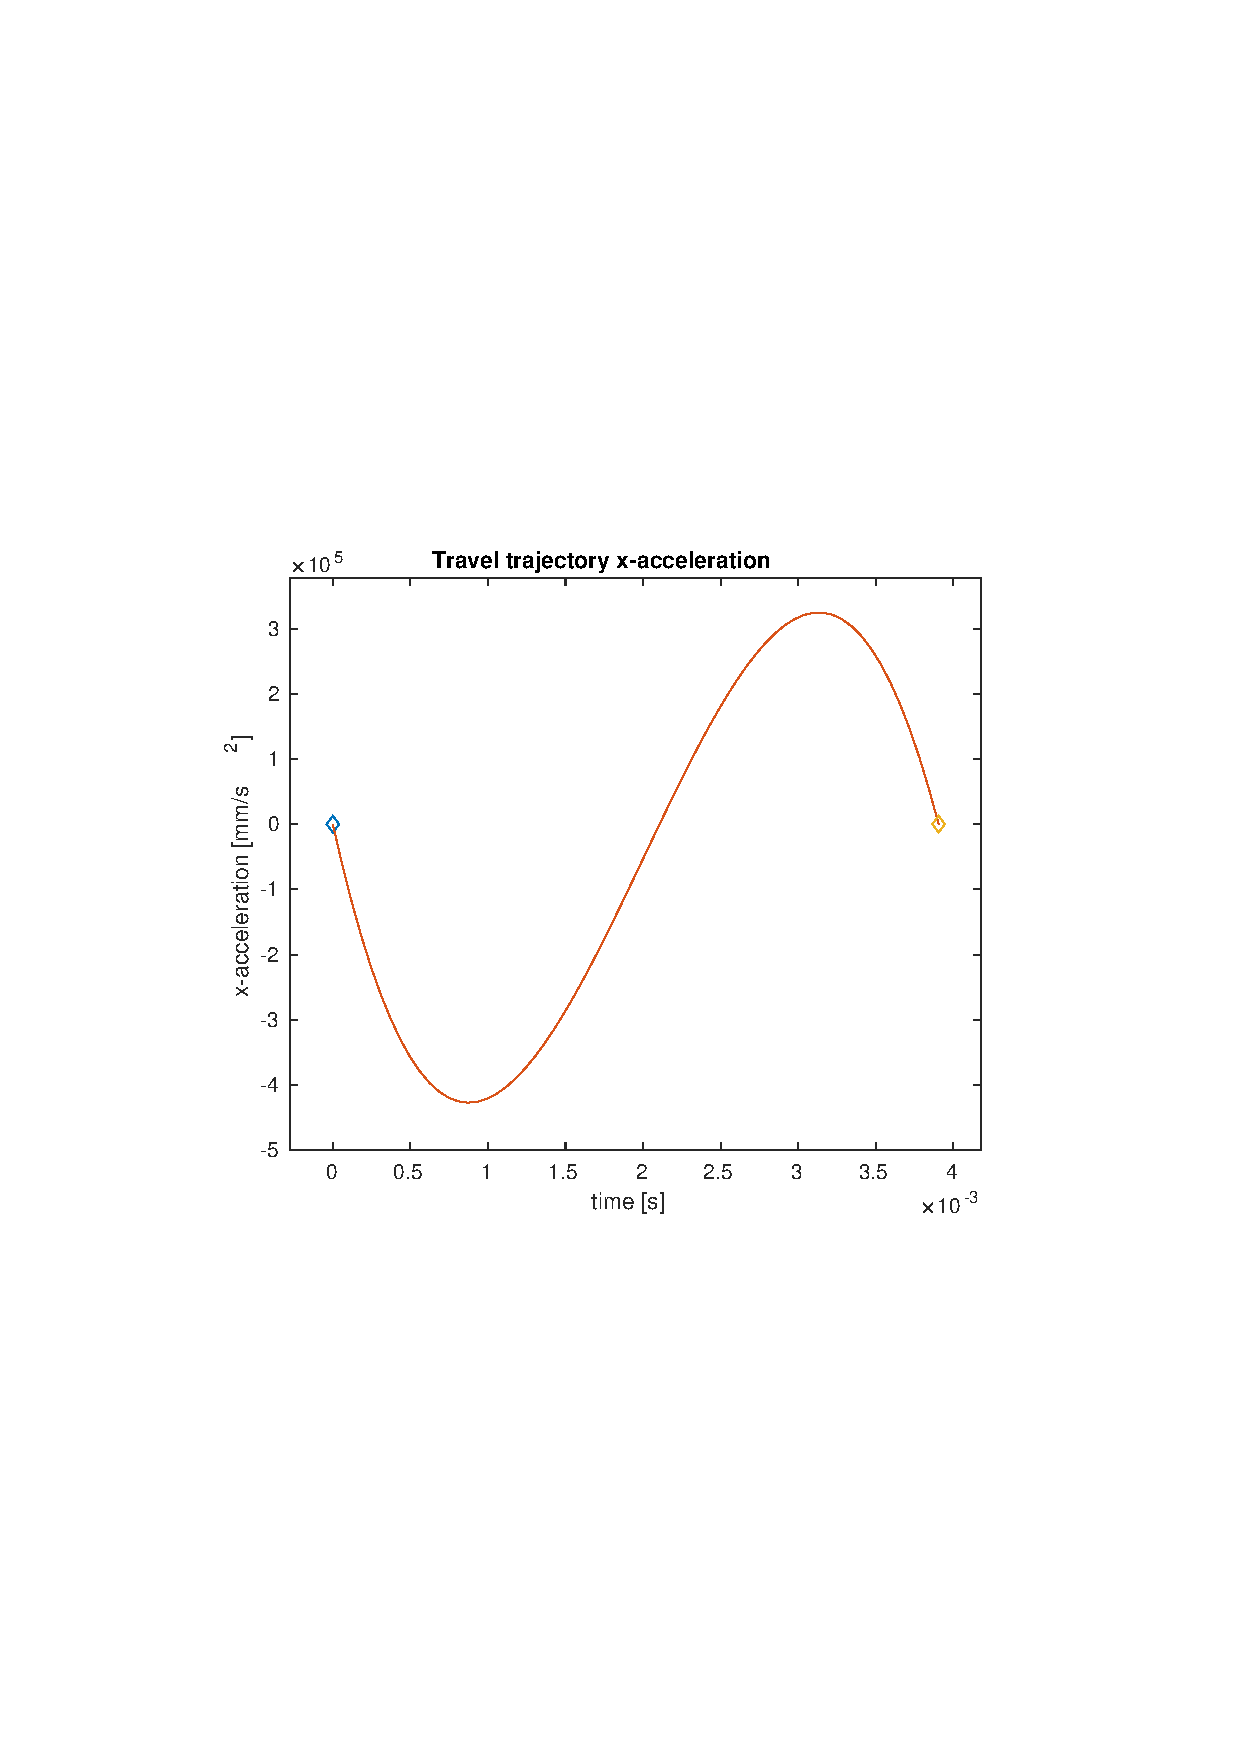
\includegraphics[clip, trim=3.5cm 9cm 4cm 9cm, width=\textwidth]{Pictures/5-traj-acc.pdf}
        \caption{The x-acceleration plotted over time, together with the end x-acceleration of the previous scan path, and the start x-acceleration of the next. This figure shows that the travel path complies with the boundary conditions on acceleration.}
        \label{fig:5-traj-acc}
    \end{subfigure}
    \caption{}
    \label{fig:5-traj-vel-acc}
\end{figure}

\section{Implementation of quintic polynomial trajectory planning}

The planning of the scanner movements for the scan trajectories happens in the slicer. Thus it makes sense to also calculate the travel trajectories there. But the trajectory planning method needs to be verified more before it is ready to be implemented in the slicer itself, so for this project it is instead implemented as a script that takes the output of the slicer and exchanges the straight positioning movements with the polynomial trajectories. All of the considerations about the how the trajectories can be implemented below are valid for both implementation by script and implementation in the slicer software.

The only way movements can be described in g-code is by giving a set of coordinates to which the laser shall move and the speed for that movement. This means the continuous polynomial needs to be split up in discrete linear segments with constant velocity. This is not much of a disadvantage, because the polynomial would need to be discretised for the digital system anyway, and g-code is a standard and sensible way to do it.

The place in the system for the trajectory planning is the same as where the calibration is implemented. So it needs to be decided which comes first. As the trajectory planning would ideally be in the slicer and the calibration would ideally be in the GLAMS, it makes sense to put the trajectory planning first. This has the advantage that the trajectory planning gets to work with the nominal values for the movement, which is the relevant metric for the limits on position and velocity, even though the calibration doesn't make a significant difference on this. The unfortunate consequence of planning the trajectories first is that a lot of extra lines are added to the g-code file during this step, so more lines will then have to be calibrated, meaning longer processing time. Since the processing time is on the order of seconds however and there are no serious time constraints, this is acceptable. The placement of the trajectory planning in the system diagram on Figure \ref{fig:system-overview} is shown of Figure \ref{fig:system-overview-w-cal-traj}.

\begin{figure}
    \centering
    \includesvg[width=0.5\linewidth]{Pictures/system-overview-w-cal-traj.svg}
    \caption{A system diagram showing where the trajectory planning is implemented. The trajectories are added before the positions are calibrated.}
    \label{fig:system-overview-w-cal-traj}
\end{figure}

\subsection{Sampling} \label{sec:trajectory-sampling}
The first step to convert the polynomials obtained in Section \ref{sec:calc-quintic-poly} to g-code is sampling. This sampling needs to be done under consideration of the hardware constraints of the scanner and the GLAMS.

\begin{itemize}
    \item The scanner has a max frequency at which it can read in new positions. The sampling frequency can not be above this limit, or expressed differently: the sampling interval, T, cannot be below the inverse of this frequency. The scanner used in Baxter communicates via the XY2-100 protocol \cite{scanner-spec}, for which this frequency is 100kHz.
    \item The GLAMS has a limited buffer size for commands. The number of g-code commands, n, used to describe the trajectory cannot exceed this buffer size. Each g-code line describes one sample interval.
\end{itemize}

These variables are connected like described in Equation \ref{eq:sample-int-g-code-line}, where n is the number of g-code lines (one for each sample), $t_1$ is the end-time of the trajectory (start-time is t=0) and T is the sample interval (the time elapsed during each g-code command).

\begin{align}
    n = \frac{t_1}{T}
    \label{eq:sample-int-g-code-line}
\end{align}

A fitting sample interval must be calculated based on these constraints. The goal is to describe the polynomial as accurately as possible, which means to aim for as low a sample interval as possible. First it is checked if the buffer size is exceeded when the sampling interval is set to be equal to the minimum scanner read interval. If not, the number of g-code lines (samples) that the polynomial is split into is set with Equation \ref{eq:no-g-code-lines}

\begin{equation}
    n = \bigg \lfloor \frac{t_1}{\text{minimum scanner read interval}} \bigg \rfloor
    \label{eq:no-g-code-lines}
\end{equation}

If setting the number of samples this way would exceed the buffer size, the best option is to use all the available buffer size, which is done by setting $n = \text{buffer size}$. In both cases the sampling interval is obtained afterwards by Equation \ref{eq:sample-int-g-code-line}. This then gives $n+1$ timestamps at which the positions must be evaluated ($t_0$ and $t_1$ included). The reason why there is one more timestamp than sample, is that the starting position is not included in the g-code, because it is assumed that the previous movement already has moved the laser there.

\subsection{Simple approach to limits on position and velocity}

Besides the sampling, the implementation is also limited in that positions and speeds are confined to certain ranges. Therefore, a way must be found to keep speeds and positions in the allowable ranges. For this, the maximum speed allowed by the scanner will be denoted as $v_{max}$ and the maximum position by $s_{max}$. This maximum position applies to both x- and y-coordinate and in both positive and negative direction.

The scanner in use in Baxter at the moment \cite{scanner-spec} has a $v_{max}$ of $\omega_{max}\alpha_{EFL} = 110 rad/s \times 423 \text{mm rad}^{-1} = 46530 mm/s$ and $s_{max}$ is $\theta_{max}\alpha_{EFL} = 0.38 rad \times 423 \text{mm rad}^{-1} = 160mm$. This section will introduce a simple but sufficient approach to keep within these limits. For example purposes $v_{max}$ and $s_{max}$ are set lower than the above hardware limits in this section.

The three main components of the script that implements this approach are two arrays of positions (one for each coordinate), an array of corresponding timestamps all of length $n+1$, and an array of speeds in between those position/time pairs of length $n$. The position arrays are straight forward to obtain by evaluating the polynomials in Equation \ref{eq:cp1} and \ref{eq:cp2} at the timestamps found in Section \ref{sec:trajectory-sampling}. The speed array is simply calculated by combining the velocity in the x and y components like shown in Equation \ref{eq:v-from-s-and-t}.

\begin{align}
    v = \sqrt{\left(\frac{\Delta s_x}{T}\right)^2 +  \left(\frac{\Delta s_y}{T}\right)^2}
    \label{eq:v-from-s-and-t}
\end{align}

The positions that exceed the scan range are reduced down to the max/min. By "reduced down" is meant that the position is set equal to $s_{max}$ for the points that would otherwise exceed the $s_{max}$ and the positions that would otherwise be less than $-s_{max}$ are set equal to $-s_{max}$. Figure \ref{fig:position-limit} shows how this position limit influences the travel path. The same example as used on Figure \ref{fig:5-traj-pos-pos} is used but shifted 1mm in the x-direction and with a position limit at 1.15mm.

\begin{figure}
    \centering
    \includesvg[width=0.85\linewidth]{Pictures/position-limit.svg}
    \caption{A travel path that is adjusted by a position limit at 1.15 mm. Each dot represents one sample (one g-code command)}
    \label{fig:position-limit}
\end{figure}

This then has the consequence that the speeds must be recalculated from the new positions to maintain that the trajectory hits the modified positions at the same timestamps as originally planned.

Then, starting from the first line segment, any elements in the speed array that exceed $v_{max}$ are set equal to $v_{max}$. For every speed that is reduced, the timestamp of the endpoint of the line segment in question and all subsequent timestamps must be updated. This will increase the total time of the travel trajectory, but this is acceptable. Keep in mind that during the extended time, the scanner moves at maximum speed, and the trajectory never leaves the scan field, so there is no risk of getting too long travel times.

\begin{figure}
    \centering
    \includesvg[width=0.85\linewidth]{Pictures/speed-limit.svg}
    \caption{The speed of a trajectory, which is limited by a speed limit at 350 mm/s. Each dot represents one sample (one for each g-code command) showing a total of 64 commands, which is the chosen buffer size.}
    \label{fig:speed-limit}
\end{figure}

This procedure will reintroduce sharp corners in the path, which were initially avoided by planning a smooth trajectory. With a high enough choice of $\bar{v}_{move}$ these will happen rarely though. In the cases where corners do appear, they are on the border of the scan field, and not next to the scan paths, which is also acceptable. The python scripts for calculating and inserting the quintic trajectories in the g-code are attached as Appendices \ref{app:quintic-planning-python} and \ref{app:traj-g-code}.

\section{Modified cubic polynomial trajectories}

The quintic polynomial trajectories are great, but the way $t_1$ is determined is heuristic and could be optimised. However trying to solve for $t_1$ based on some extra condition becomes very tricky with two fifth order polynomials. The question is then if it is possible to make do, with a simpler function. An option for simplification is that the boundary conditions on velocity and acceleration in the beginning of the travel trajectory are probably dispensable. The mirrors will have a harder time trying to track an instant change in velocity in the beginning of the travel trajectory. That is acceptable though, as long as they are tracking the trajectory well when the next scan trajectory begins. Skipping these two boundary conditions on each of the variables opens the option to use a third order polynomial instead of the fifth order polynomial. Using third order polynomials in trajectories is nothing new, but the reason it is called "modified" here is that there is one boundary condition in the beginning and three in the end, rather than two (position and velocity) in both beginning and end.

With this third order polynomial, the idea is to determine $t_1$ in a different way than the heuristic distance-based one used for the fifth order polynomial. A weakness of the distance-based method was that the speed sometimes overshot the maximum speed of the scanner and had to be limited in the implementation. Therefore a promising strategy seems to be to derive $t_1$ from this speed limit. More specifically, to choose $t_1$ so that the maximum speed of the trajectory always exactly reaches the speed limit. Not only does this prevent an overshoot of the speed but it also ensures that the system makes use of the available velocity range. This makes sure no time is wasted by travelling slower than necessary and the resulting trajectories would be optimal in that sense.

To chose $t_1$ in such a way that the maximum speed of the trajectory is exactly the speed limit, it must first be determined where in the trajectory the maximum speed occurs. Since the position is a third order polynomial function of time, the velocity must be a second order polynomial function of time. Furthermore, since the acceleration must be 0 at $t_1$ according to the boundary condition, the only local extrema of the velocity must occur at $t=t_1$. Since second order polynomials have at most one local extrema this means the global extrema of the velocity must occur at either $t_0$ or $t_1$. The velocity at $t_1$ is already known - it is also given by the boundary condition and equal to the velocity of the following scan trajectory. The programmed speed of a scan trajectory will never be greater than the speed limit, so the maximum speed must occur at $t_0$. This gives Equation \ref{eq:cubic-v0} in addition to the Equations \ref{eq:cubic-s0}, \ref{eq:cubic-s1}, \ref{eq:cubic-v1} and \ref{eq:cubic-a1} from the boundary conditions.

\begin{align}
    s_0 &= \beta_0 \label{eq:cubic-s0}\\
    s_1 &= \beta_0 + \beta_1 t_1 + \beta_2 t_1^2 + \beta_3 t_1^3 \label{eq:cubic-s1}\\
    \pm v_{max} = v_0 &= \beta_1 \label{eq:cubic-v0}\\
    v_1 &= \beta_1 + 2\beta_2 t_1 + 3 \beta_3 t_1^2 \label{eq:cubic-v1} \\
    0 = a_1 &= 2\beta_2 + 6\beta_3 t_1 \label{eq:cubic-a1}
\end{align}

The first goal is to solve for $t_1$. Throughout the derivation it will be used that $t_1 > t_0 = 0$.
The derivation begins by multiplying Equation \ref{eq:cubic-a1} by $-t_1/2$ on both sides and add it to Equation \ref{eq:cubic-v1} to obtain Equation \ref{eq:cubic-beta2}.

\begin{align}
    v_1 &= \beta_1 + \beta_2 t_1 <=> \\
    \beta_2 &= \frac{v_1 - \beta_1}{t_1} \label{eq:cubic-beta2}
\end{align}

Now Equation \ref{eq:cubic-s1} is multiplied by three and Equation \ref{eq:cubic-a1} is multiplied by $-t_1^2/2$ and the two resulting equations are added, side by side. Then the expression for $\beta_2$ from Equation \ref{eq:cubic-beta2} is substituted in which after some simplification gives Equation \ref{eq:cubic-3s1} which can then be solved for $t_1$.

\begin{align}
    3s_1 &= 3\beta_0 + (2v_1 + \beta_1)t_1 \label{eq:cubic-3s1} \\
    t_1 &= \frac{3s_1-3\beta_0}{2v_1 + \beta_1}
\end{align}

Lastly, substituting values for $\beta_0$ and $\beta_1$ from Equations \ref{eq:cubic-s0} and \ref{eq:cubic-v0} produces Equation \ref{eq:cubic-t1}, which is an expression for $t_1$ as a function of $v_{max}$ and known boundary conditions.

\begin{align}
    t_1 &= \frac{3(s_1-s_0)}{2v_1 \pm v_{max}} \label{eq:cubic-t1}
\end{align}

The only thing left to settle is whether the velocity at $t=t_0$ should be $+v_{max}$ or $-v_{max}$. This decision must be based on which of the options will result in a (positive) solution for $t_1$. The different cases are presented in Table \ref{tab:t1-vs-vmax}.

\begin{table}[]
    \centering
    \begin{tabular}{c|c|c|c}
        $s_1 - s_0$ & $v_1$ & $v_{max} - 2v_1$ & $\pm v_{max}$ \\ \hline
        + & + & + & + \\  \hline
        + & + & - & $\pm$ \\ \hline
        + & - & + & + \\ \hline
        + & - & - & Ø \\ \hline
        - & + & + & - \\ \hline
        - & + & - & Ø \\ \hline
        - & - & + & - \\ \hline
        - & - & - & $\pm$
    \end{tabular}
    \caption{The three leftmost columns of the table give information about the signs of different parts of the expression on the right side of Equation \ref{eq:cubic-t1}. Based on this, the rightmost column notes which of options $+v_{max}$ or $-v_{max}$ will give a positive $t_1$. "Ø" means neither of the options work, and $\pm$ means both work.}
    \label{tab:t1-vs-vmax}
\end{table}

Two conclusions can be drawn from this table. First off, the cases in which there is no solution for $t_1$ are both when $v_{max} \leq 2v_1$. Therefore, this trajectory planning method will only work if $v_{max} > 2v_1$, but luckily this is almost always the case. To this must be added that since the speed limit given in the scanner specifications might be for the combination of x and y speed, the speed limit $v_{max}$ for each of the coordinates must be less than $1/\sqrt{2}$ times the scanner speed limit. This will avoid breaching the scanner speed limit even if both the scanner moves at $v_{max}$ in both x- and y-direction. This then gives that $1/\sqrt{2} \text{scanner speed limit} > v_{max} > 2v_1$ or as a rule of thumb Equation \ref{eq:speed-limit-v1}.

\begin{align}
    \text{scan trajectory speed} \leq \frac{\text{scanner speed limit}}{3} \label{eq:speed-limit-v1}
\end{align}

Note that this limitation is specific to this type of cubic trajectory and that the quintic trajectories are not liable to it.

The second fact that can be concluded from Table \ref{tab:t1-vs-vmax} is about the sign of $\pm v_{max}$. The table shows that choosing the same sign for $\pm v_{max}$ as the sign of $s_1 - s_0$ will always give a valid $t_1$ if there's compliance with the above conditions on the magnitude of $v_{max}$.

Since a trajectory is calculated for both x- and y-motion, two possibly different values for $t_1$ are found. This is a problem as both motions should arrive at the next scan trajectory at the same time. This will be resolved later but first it is necessary to take a look at the next step: How to determine the polynomial coefficients from the boundary conditions. This is done in a very similar way as for the quintic polynomials. The Equations \ref{eq:cubic-s0}, \ref{eq:cubic-s1}, \ref{eq:cubic-v1} and \ref{eq:cubic-a1} are solved for $\beta_0$, $\beta_1$, $\beta_2$ and $\beta_3$. This gives the solutions in Equations \ref{eq:cubic-beta0} through \ref{eq:cubic-beta3}.

\begin{align}
    \beta_0 &= s_0 \label{eq:cubic-beta0} \\
    \beta_1 &= -\frac{3s_0 - 3s_1 + 2t_1 v_1}{t_1} \label{eq:cubic-beta1} \\
    \beta_2 &= \frac{3(s_0 - s_1 + t_1 v_1)}{t_1^2} \\
    \beta_3 &= -\frac{s_0 - s_1 + t_1v_1}{t_1^3} \label{eq:cubic-beta3}
\end{align}

From Equation \ref{eq:cubic-beta1} it can be verified that setting $t_1$ with the formula found earlier in Equation \ref{eq:cubic-t1} will result in $\beta_1 = v_0 = \pm v_{max}$. But this expression for $\beta_1$ also shows what to do about the two different values for $t_1$. First it needs to be rearranged like shown in Equation \ref{eq:cubic-beta1-alt}

\begin{align}
    \beta_1 = v_0 = \pm v_{max} = \frac{3(s_1 - s_0)}{t_1} - 2 v_1 \label{eq:cubic-beta1-alt}
\end{align}

Because $\pm v_{max}$ is chosen to have the same sign as $s_1-s_0$ it can be derived that increasing $t_1$ would result in a $v_{max}$ and thus $v_0$ of smaller magnitude. This can be seen by reasoning about the two cases. Either $s_1-s_0$ is positive meaning $v_{max}$ is positive, which in turn means the whole right hand side of the equation is positive. If $t_1$ would be increased, the magnitude of the fraction would decrease. The other term is unaffected, meaning the magnitude of the whole right hand side would decrease, which then ends up meaning the magnitude of $v_0$ would be lower than for the original $t_1$. This means that choosing the greater of the two $t_1$'s found from the two sets of boundary conditions and applying it when determining the trajectories in both x- and y-direction ensures that the maximum speed of neither of the trajectories climbs over $v_{max}$. This also solves the issue that one of the $t_1$'s found will often be zero (when one of the coordinates stays the same) which would be a problem when determining the $\beta$-coefficients.

The same example as was presented for the quintic trajectory in Figures \ref{fig:5-traj-pos} and \ref{fig:5-traj-vel-acc} but now with modified cubic trajectories instead is presented on Figures \ref{fig:3-traj-pos} and \ref{fig:3-traj-vel-acc}.

\begin{figure}[hp]
    \centering
    \begin{subfigure}{0.72\textwidth}  
        \centering 
        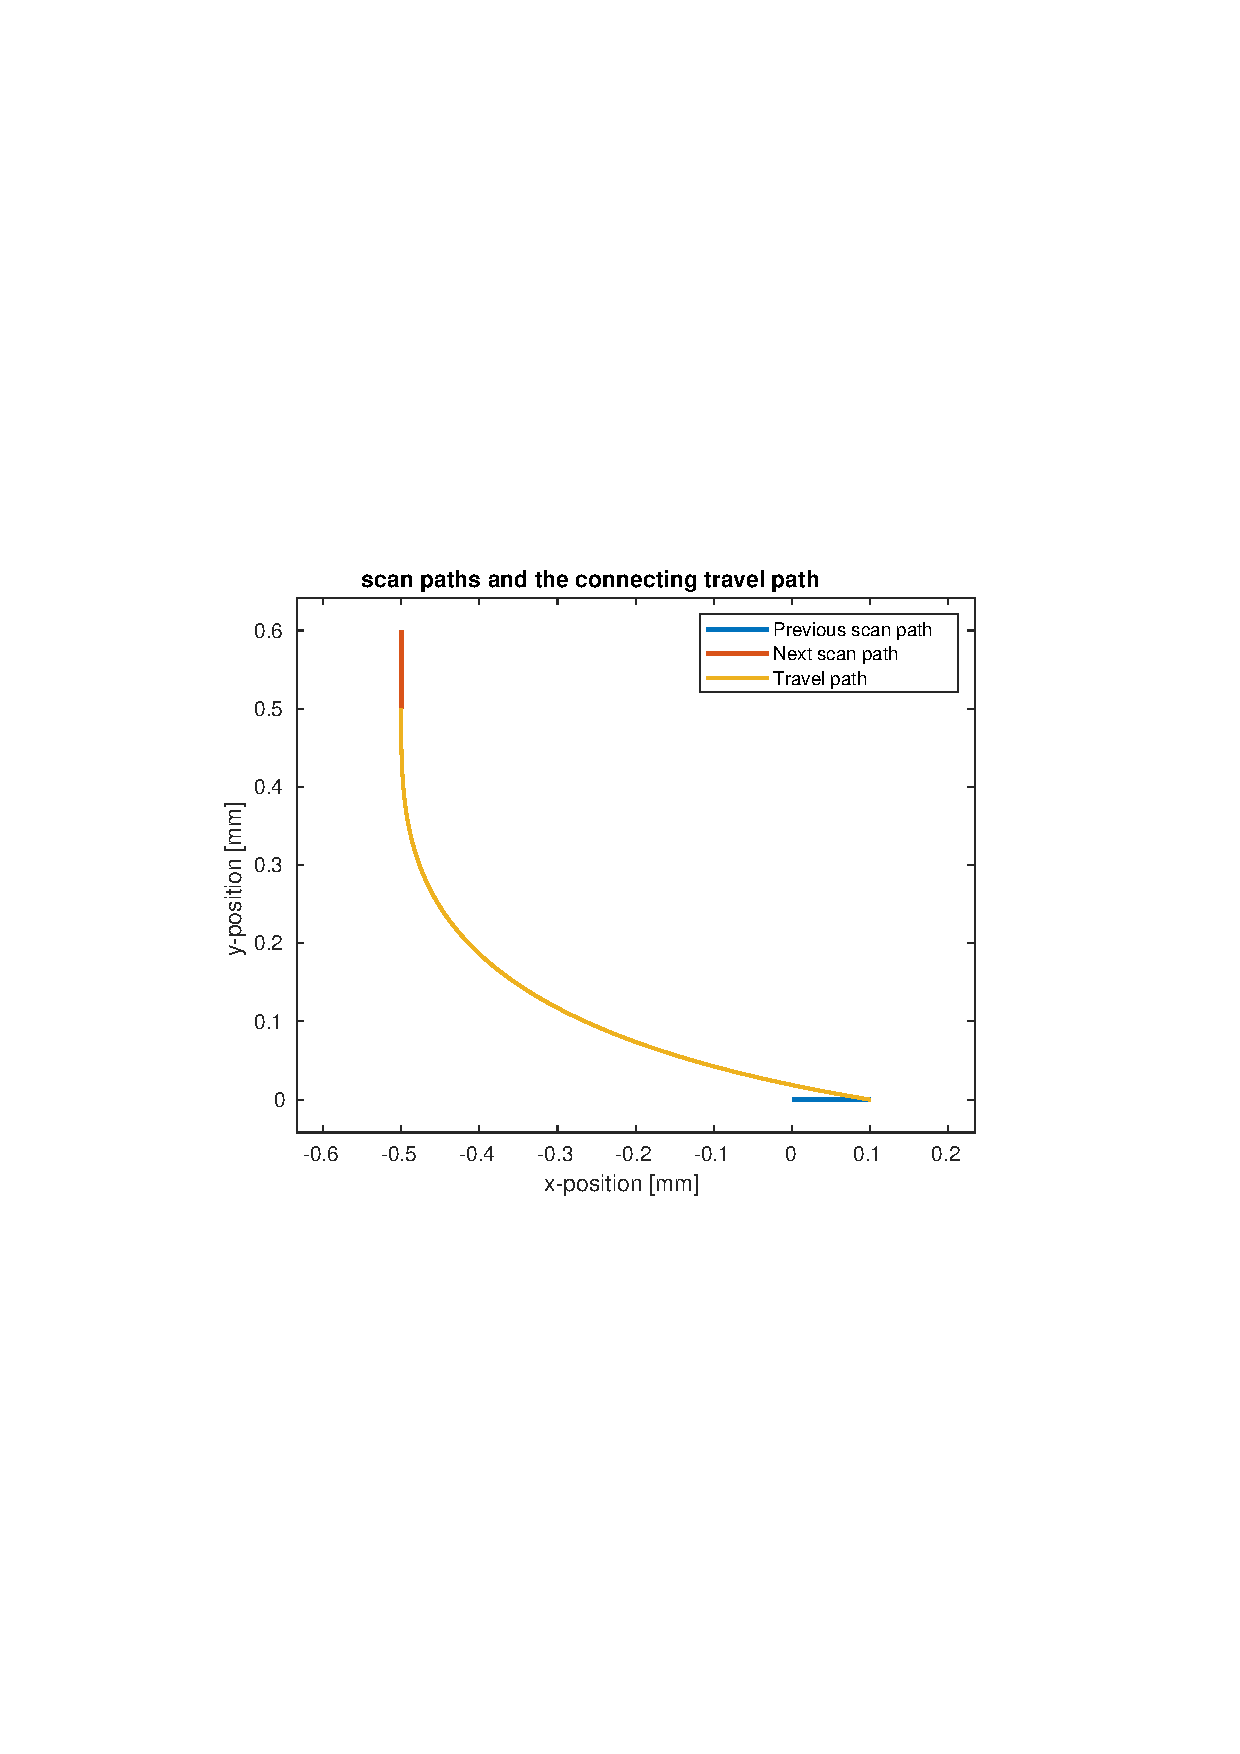
\includegraphics[clip, trim=3.5cm 9cm 4cm 9cm, width=\textwidth]{Pictures/3-scan-travel-path.pdf}
        \caption{An example of two scan paths and a cubic travel trajectory path that brings the laser from one to the other}    
        \label{fig:3-traj-pos-pos}
    \end{subfigure}
    \vskip\baselineskip
    \begin{subfigure}{0.72\textwidth}   
        \centering 
        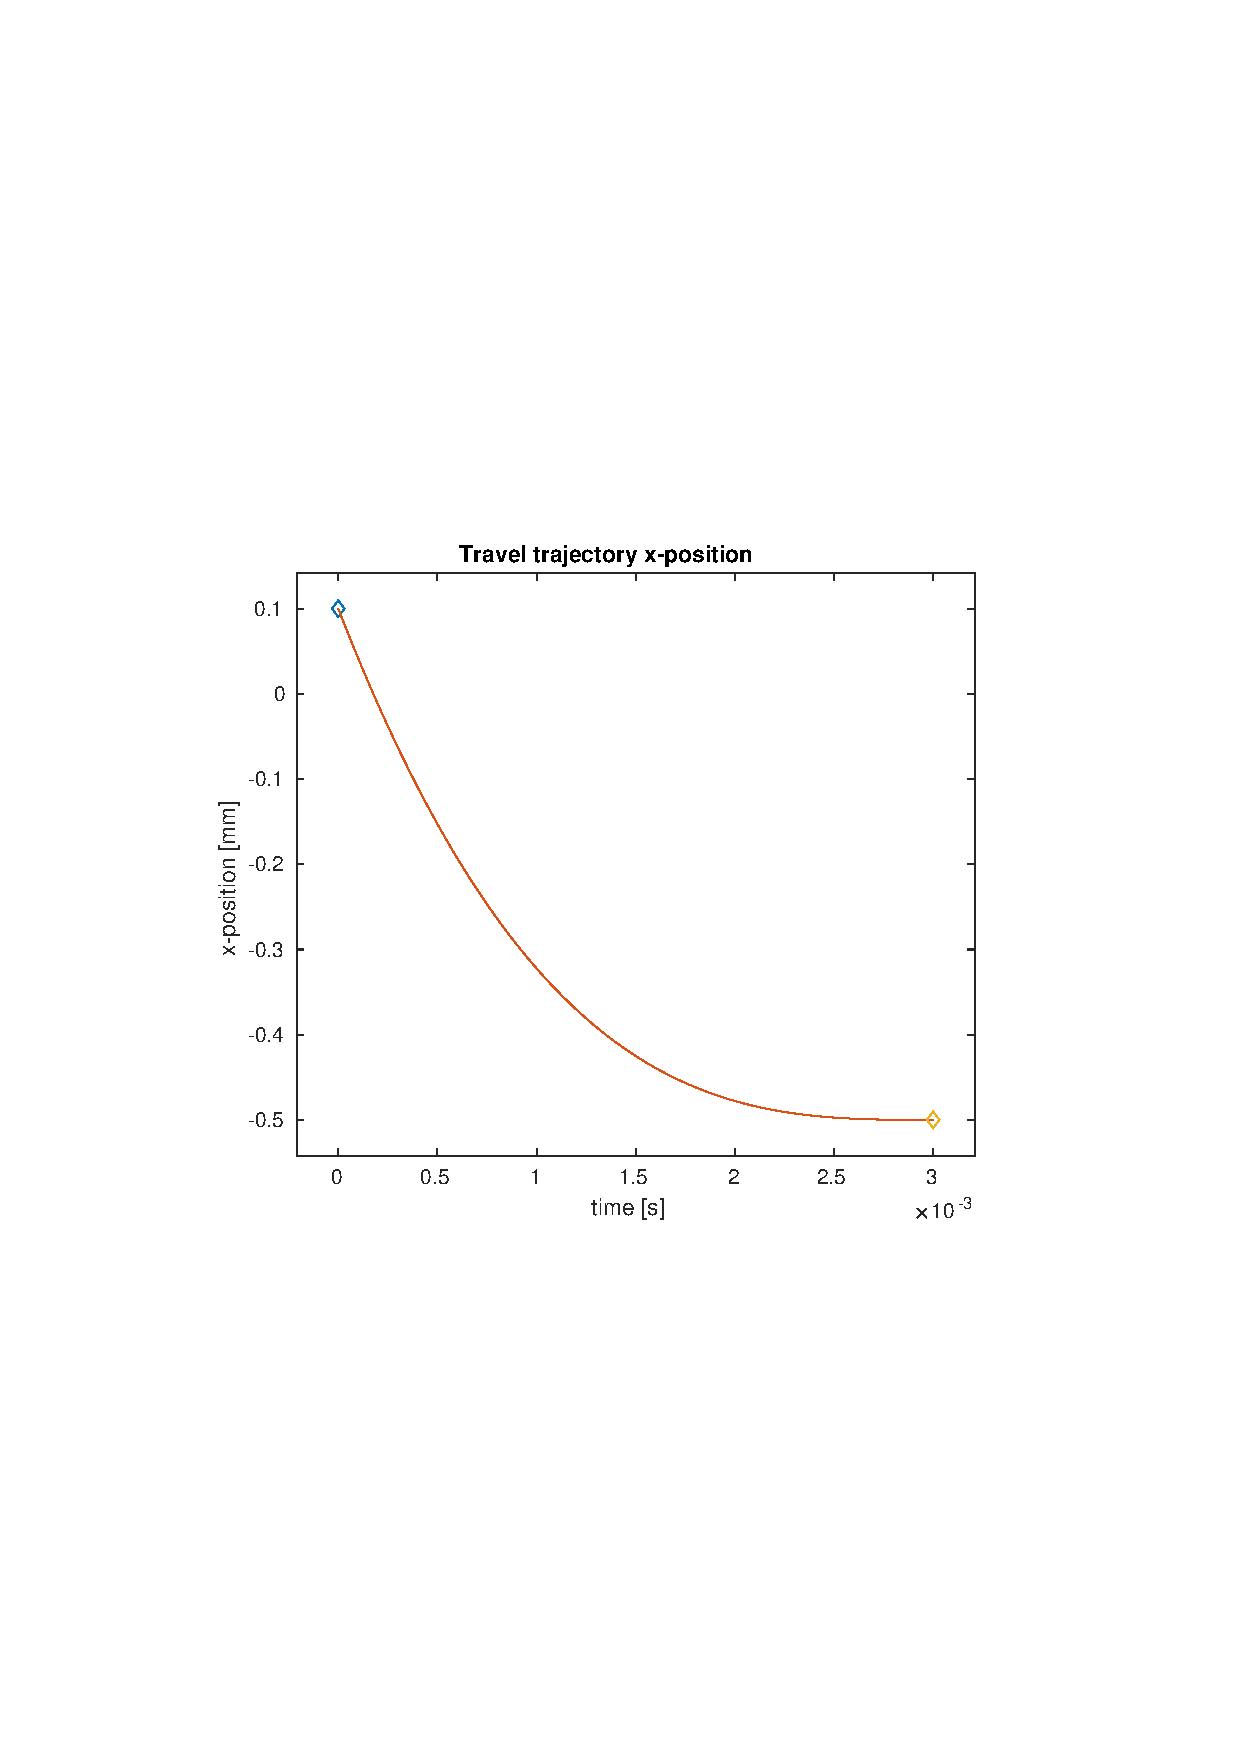
\includegraphics[clip, trim=3.5cm 9cm 4cm 9cm, width=\textwidth]{Pictures/3-traj-pos.pdf}
        \caption{The x-position plotted over time, together with the end x-position of the previous scan path, and the start x-position of the next. This figure shows that the cubic trajectory complies with the boundary conditions on position.}
        \label{fig:3-traj-pos-t}
    \end{subfigure}
    \caption{}
    \label{fig:3-traj-pos}
\end{figure}

\begin{figure}[hp]
    \centering
    \begin{subfigure}{0.72\textwidth}   
        \centering 
        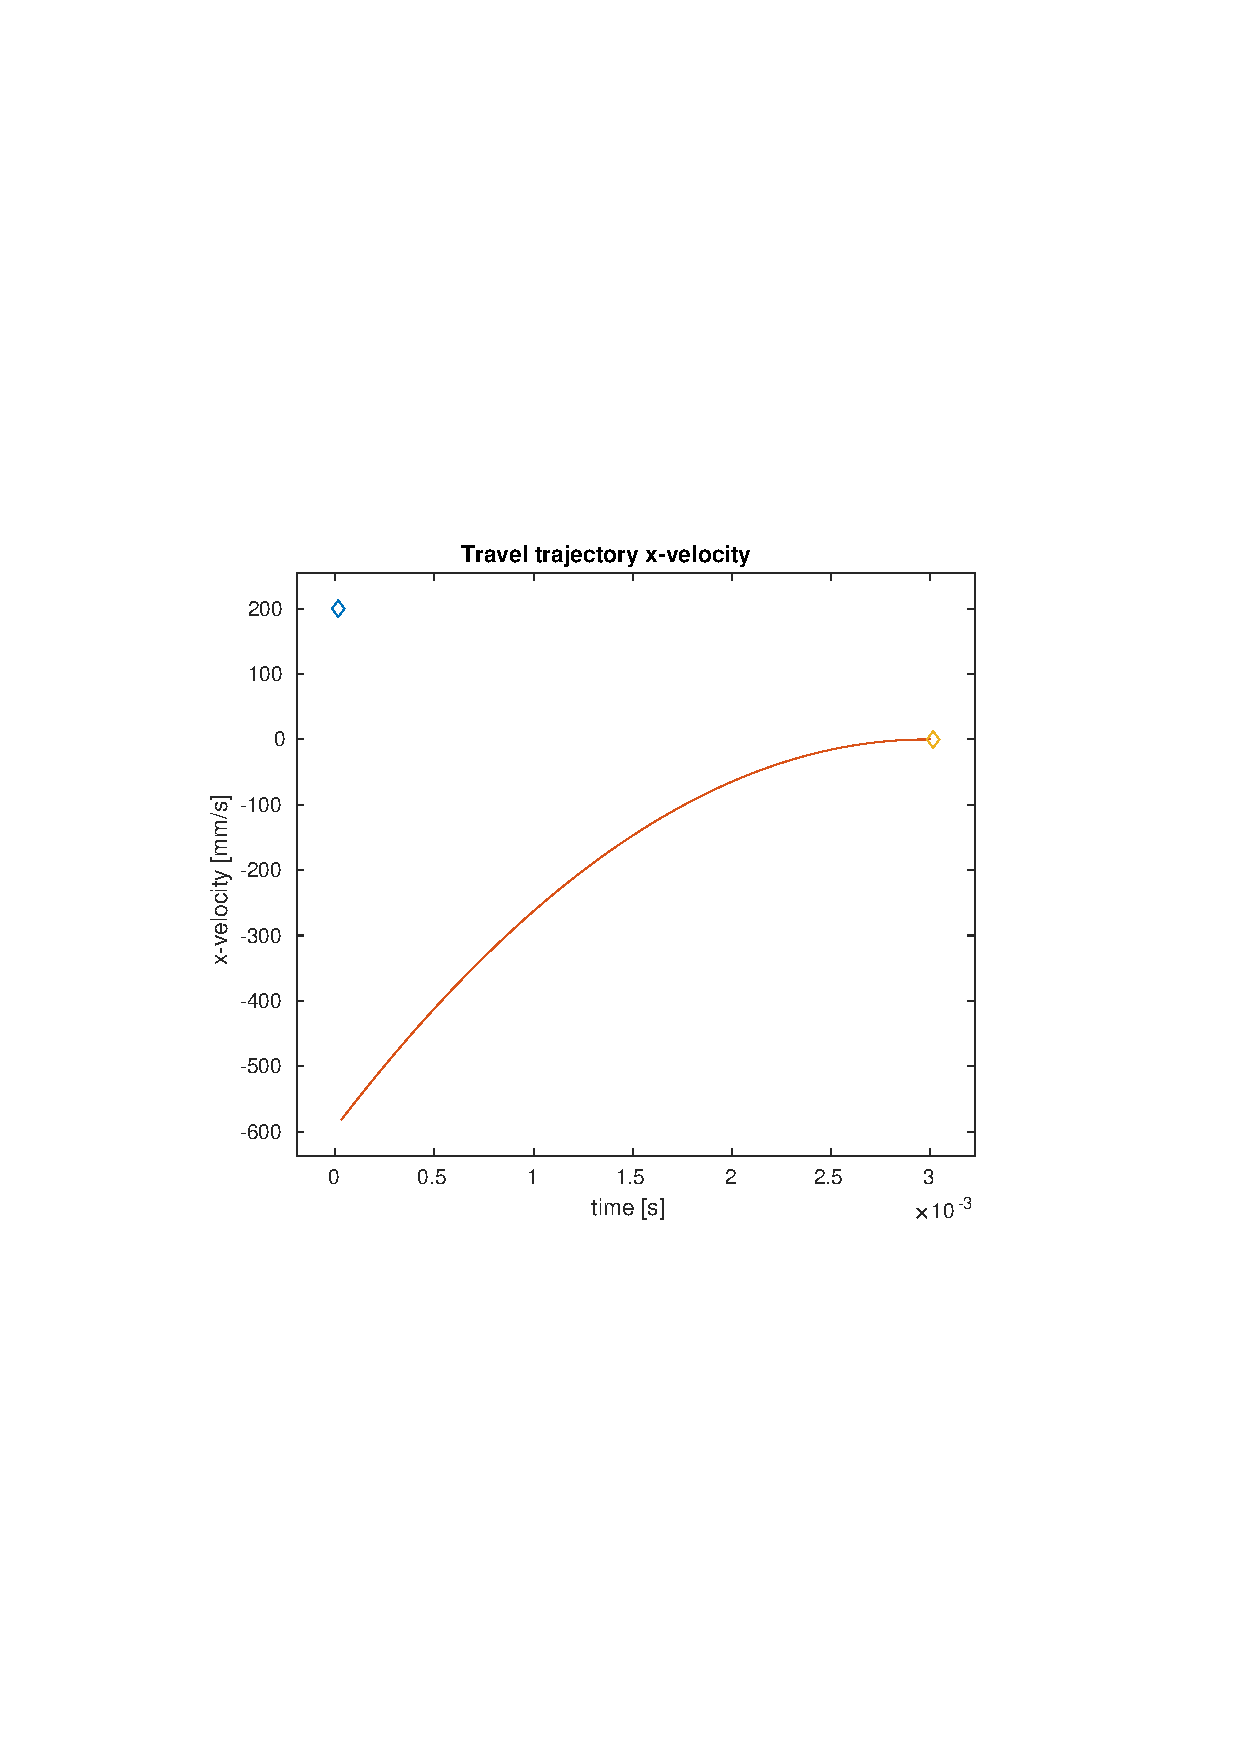
\includegraphics[clip, trim=3.5cm 9cm 4cm 9cm, width=\textwidth]{Pictures/3-traj-vel.pdf}
        \caption{The x-velocity plotted over time, with the end x-velocity of the previous scan path, and the start x-velocity of the next. Note that the cubic trajectory doesn't start at the speed of the previous scan path, but at 600mm/s which is the speed limit for this example. Note also that the velocity follows a parabola and ends at the extrema}    
        \label{fig:3-traj-vel}
    \end{subfigure}
    \vskip\baselineskip
    \begin{subfigure}{0.72\textwidth}   
        \centering 
        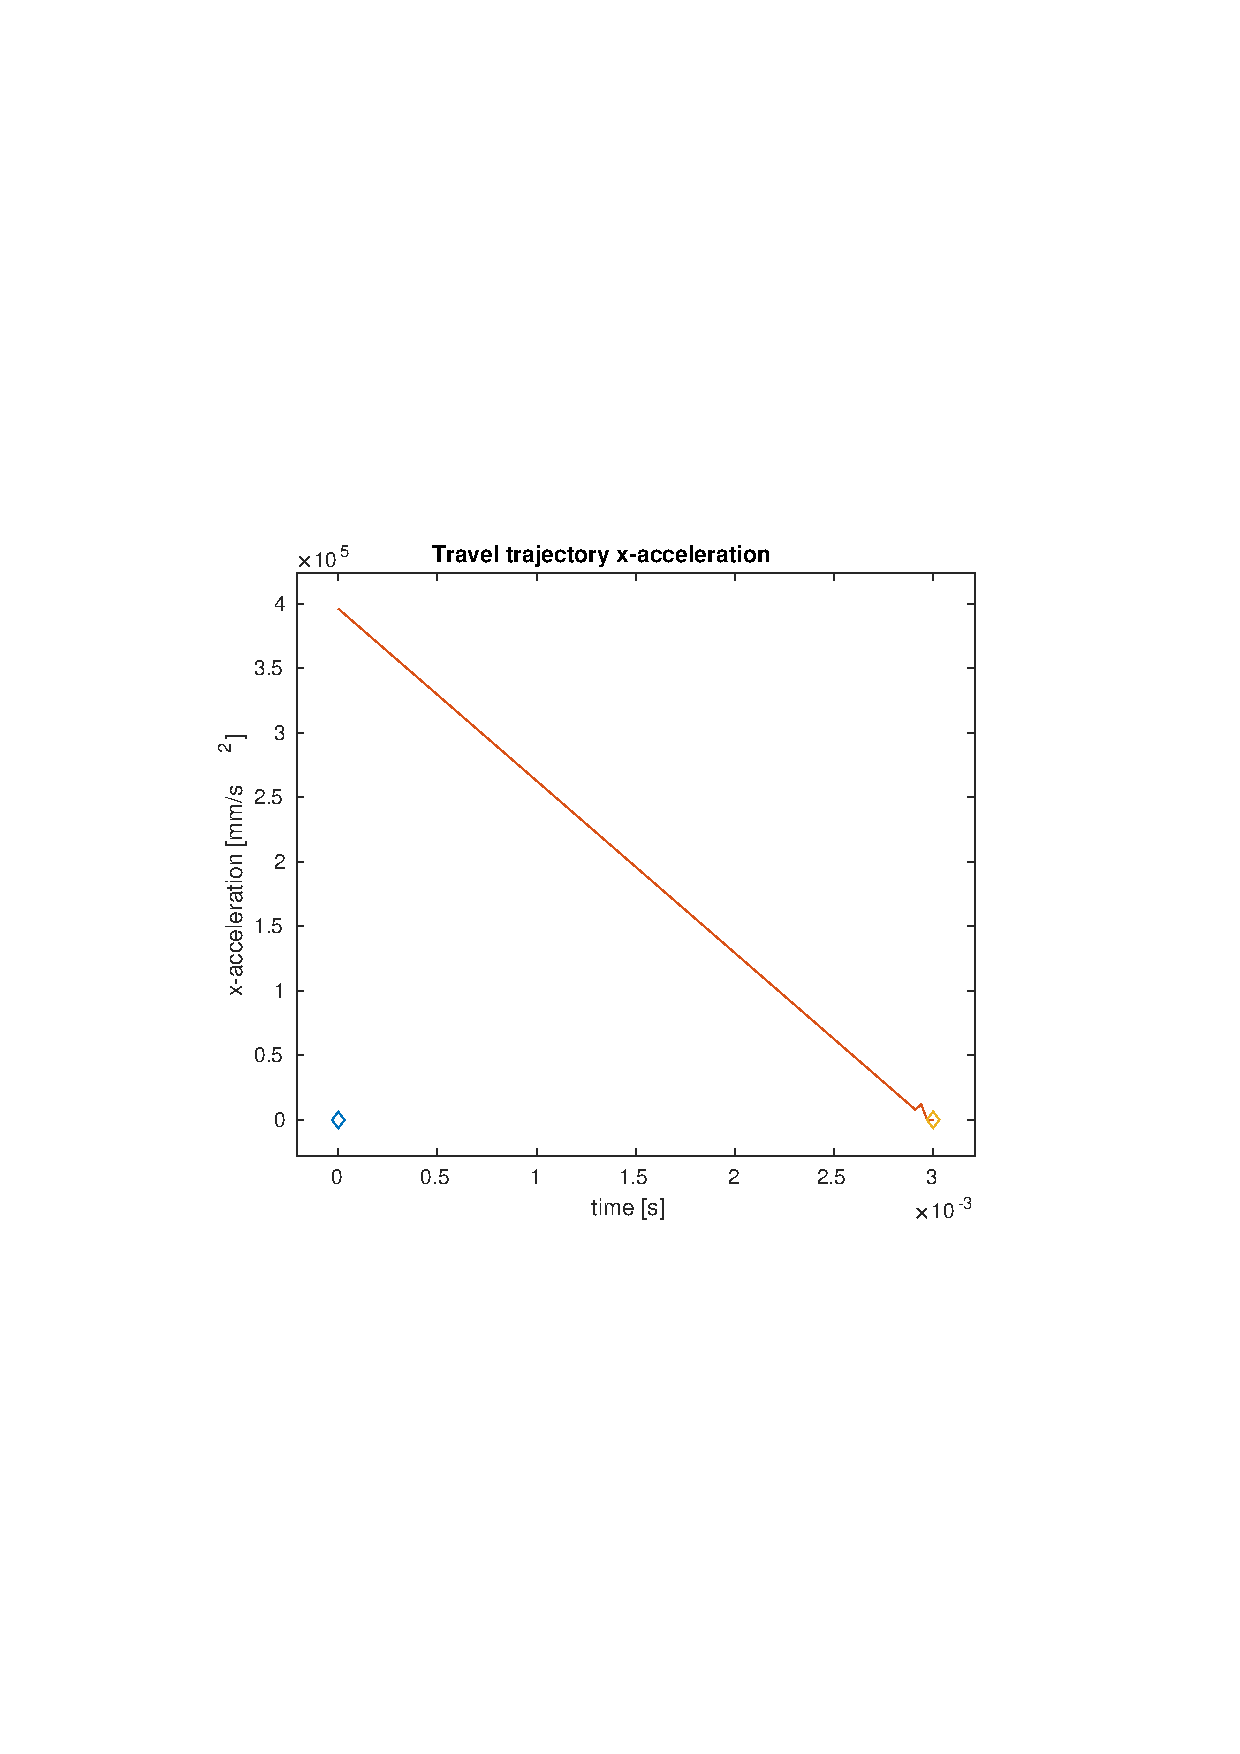
\includegraphics[clip, trim=3.5cm 9cm 4cm 9cm, width=\textwidth]{Pictures/3-traj-acc.pdf}
        \caption{The x-acceleration plotted over time, together with the end x-acceleration of the previous scan path, and the start x-acceleration of the next. This figure shows that there only is a boundary conditions on acceleration for the end of the cubic trajectory, not for the beginning.}
        \label{fig:3-traj-acc}
    \end{subfigure}
    \caption{}
    \label{fig:3-traj-vel-acc}
\end{figure}

The implementation of the cubic polynomial trajectories can be done in exactly the same matter as the for quintic polynomial trajectories. The same procedure for time discretisation works and likewise for the position limiting. No speed limiting step is needed since the trajectory is already designed analytically to not exceed the maximum speed and limiting the positions never increases the speed of any of the segments. The python script for calculating the cubic trajectories is attached as Appendix \ref{app:cubic-planning-python}. The same script as was used for the quintic trajectories, can be used to insert the cubic trajectories in the g-code (Appendix \ref{app:traj-g-code}).

\section{Testing the trajectories}

An experiment was devised to test if the trajectories work in practice. To be able to see the travel trajectories, where the laser would normally be off, the laser was connected to a function generator instead of the GLAMS. This function generator was set to output a 250 Hz square wave with a duty-cycle of 20\%. A g-code file describing four sets of four lines, each set with a different scan trajectory velocity was prepared to showcase the behaviour of the trajectories at different velocities. The four different velocities were 250 mm/s, 500 mm/s, 750 mm/s and 1000 mm/s. This means that the laser travels 1 mm, 2 mm, 3 mm and 4 mm in one period of the square wave for the different velocities respectively.

Both the quintic and cubic trajectories were calculated with the parameters presented in Table \ref{tab:traj-test-params} with the exception that the average speed for the travel trajectories is not used when planning the cubic trajectories.

\begin{table}[]
    \centering
    \begin{tabular}{c|c|l}
        Quantity & Value & Unit \\ \hline
        Position limit & 57.7 & mm \\
        Speed limit & 3000 & mm/s \\
        Minimum time per g-code line & 10 & $\mu$ s \\
        average speed for travel trajectories & 300 & mm/s \\
        Maximum no. line segments & 31 & \\
    \end{tabular}
    \caption{The parameters used when calculating the trajectories for the experiment.}
    \label{tab:traj-test-params}
\end{table}

\subsection{Trajectory planning results}

The results of the runs can be seen on Figures \ref{fig:5th-order-high-contrast} and \ref{fig:3rd-order-high-contrast}.

\begin{figure}
    \centering
    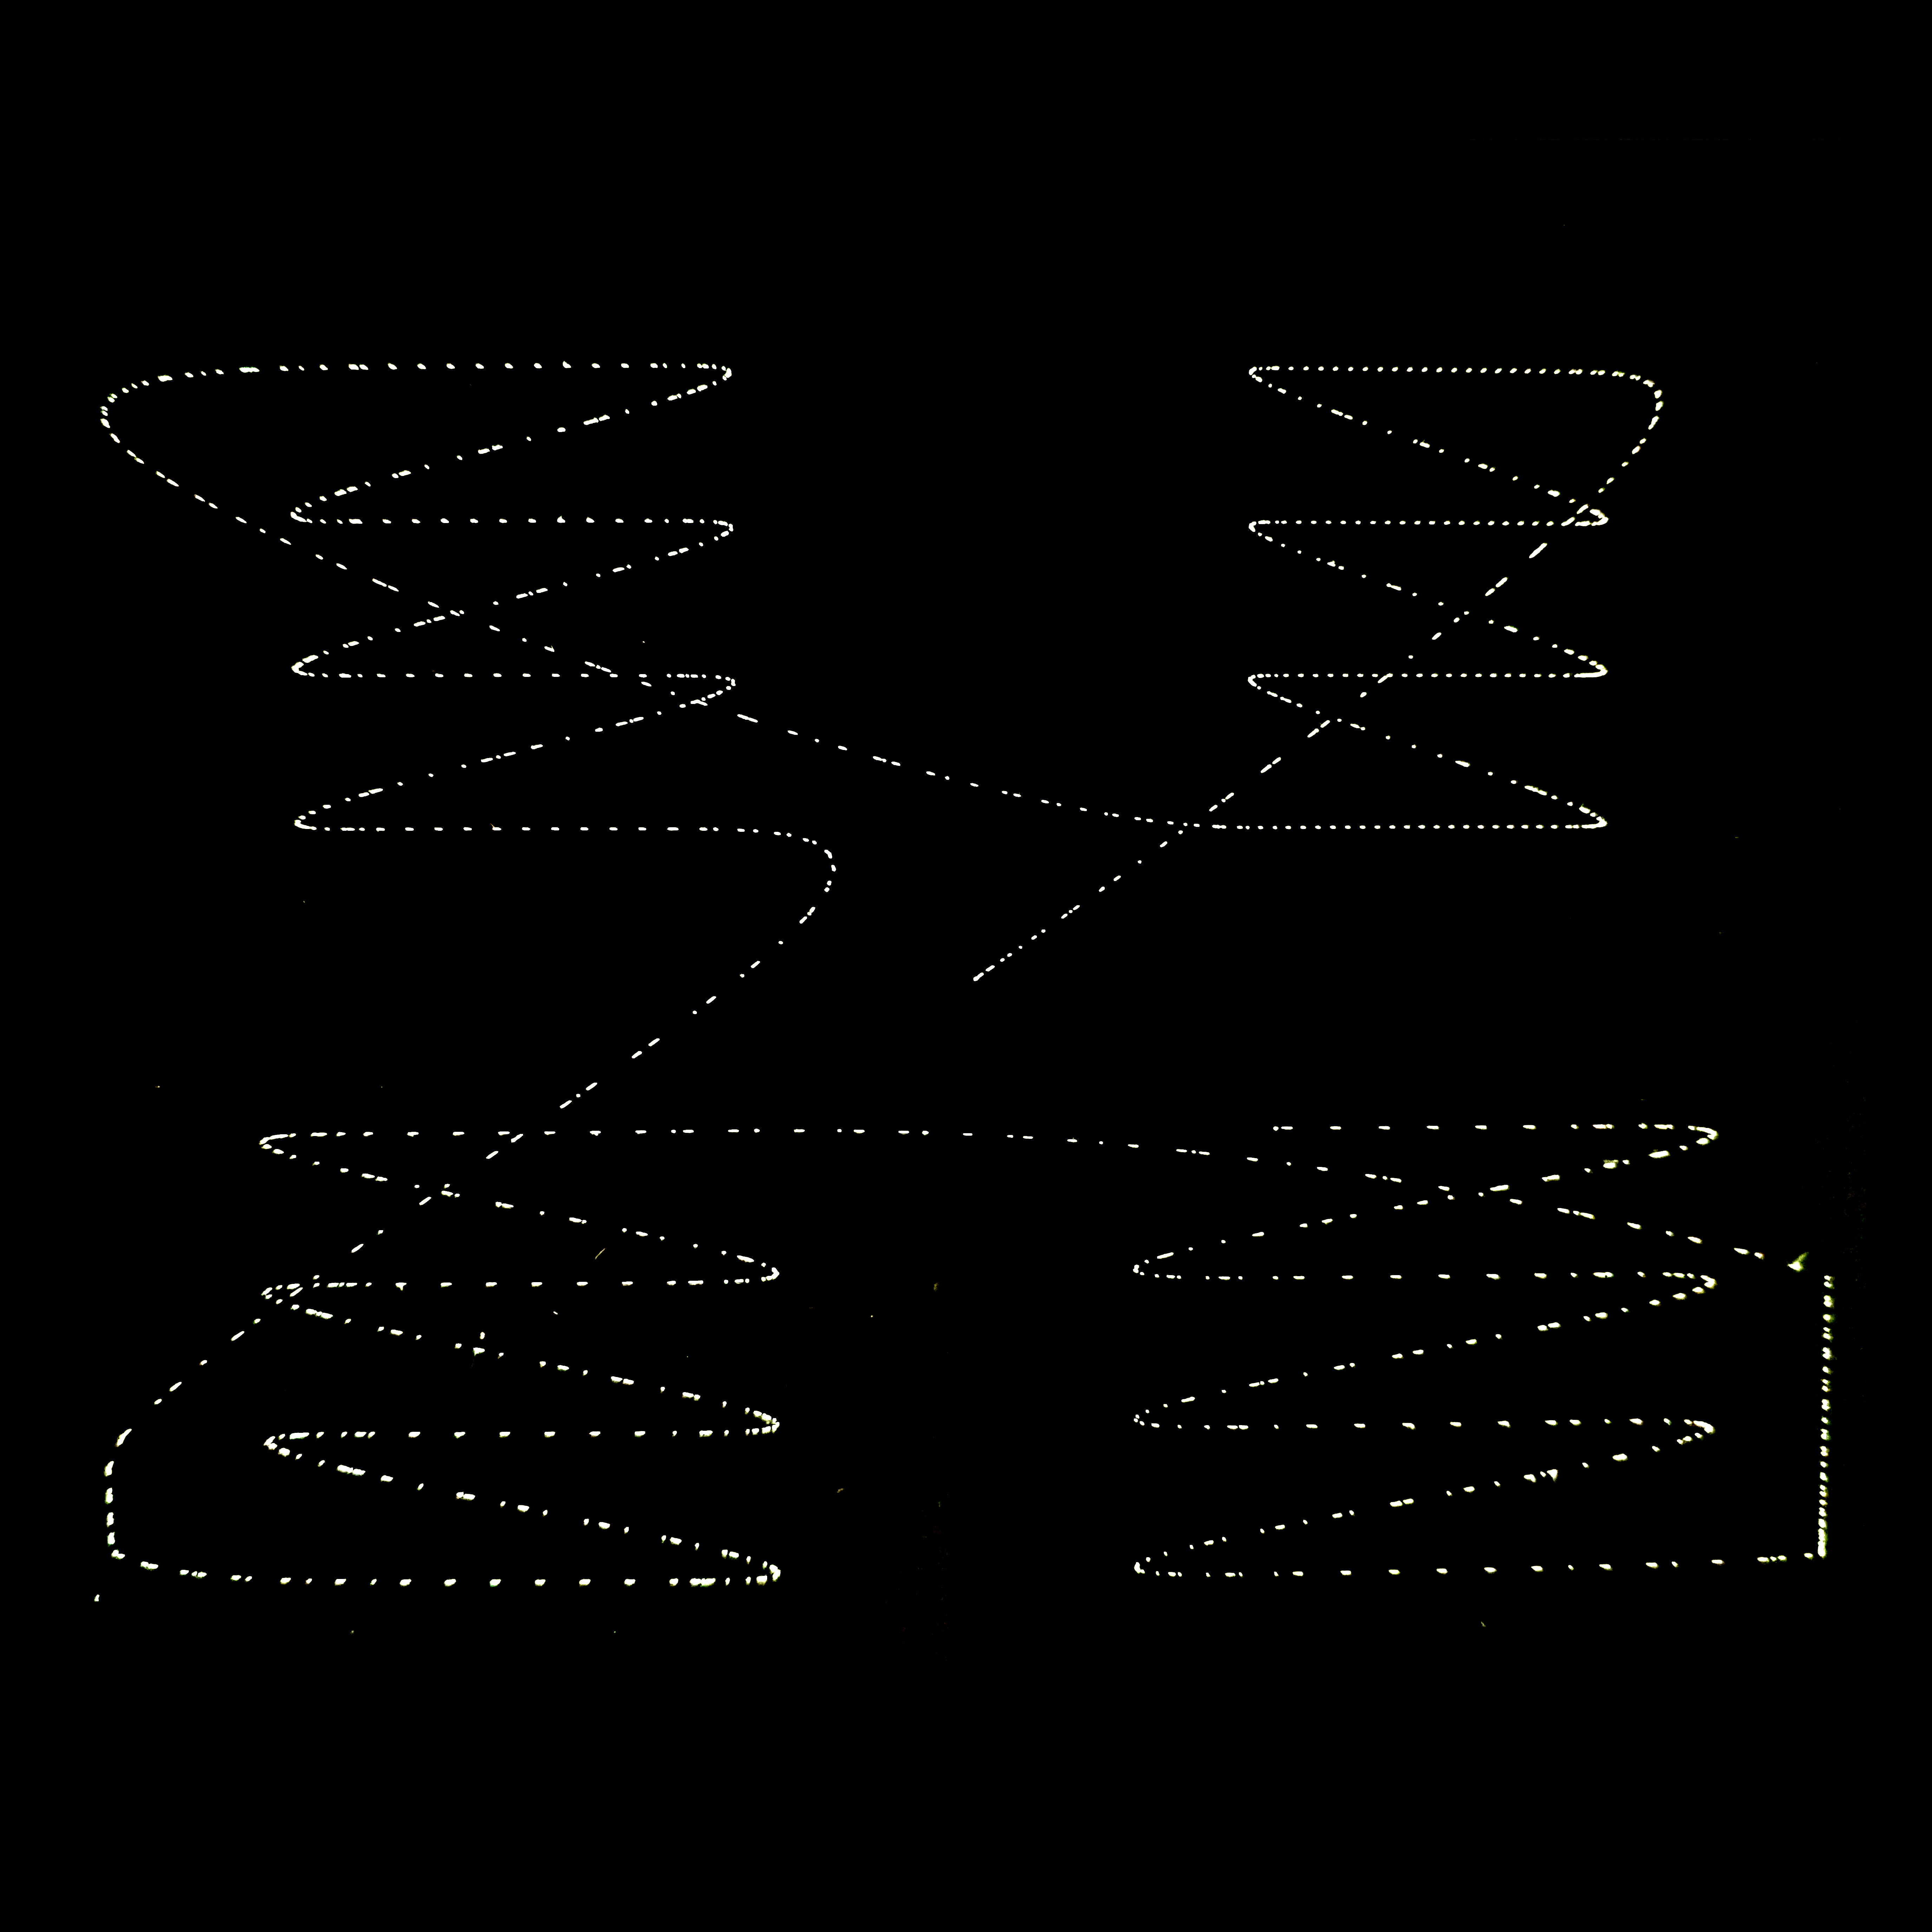
\includegraphics[width=\linewidth]{Pictures/5th-order-high-contrast.png}
    \caption{A series of scan paths and their 5th-order connecting travel trajectories traced with a pulsed laser}
    \label{fig:5th-order-high-contrast}
\end{figure}

\begin{figure}
    \centering
    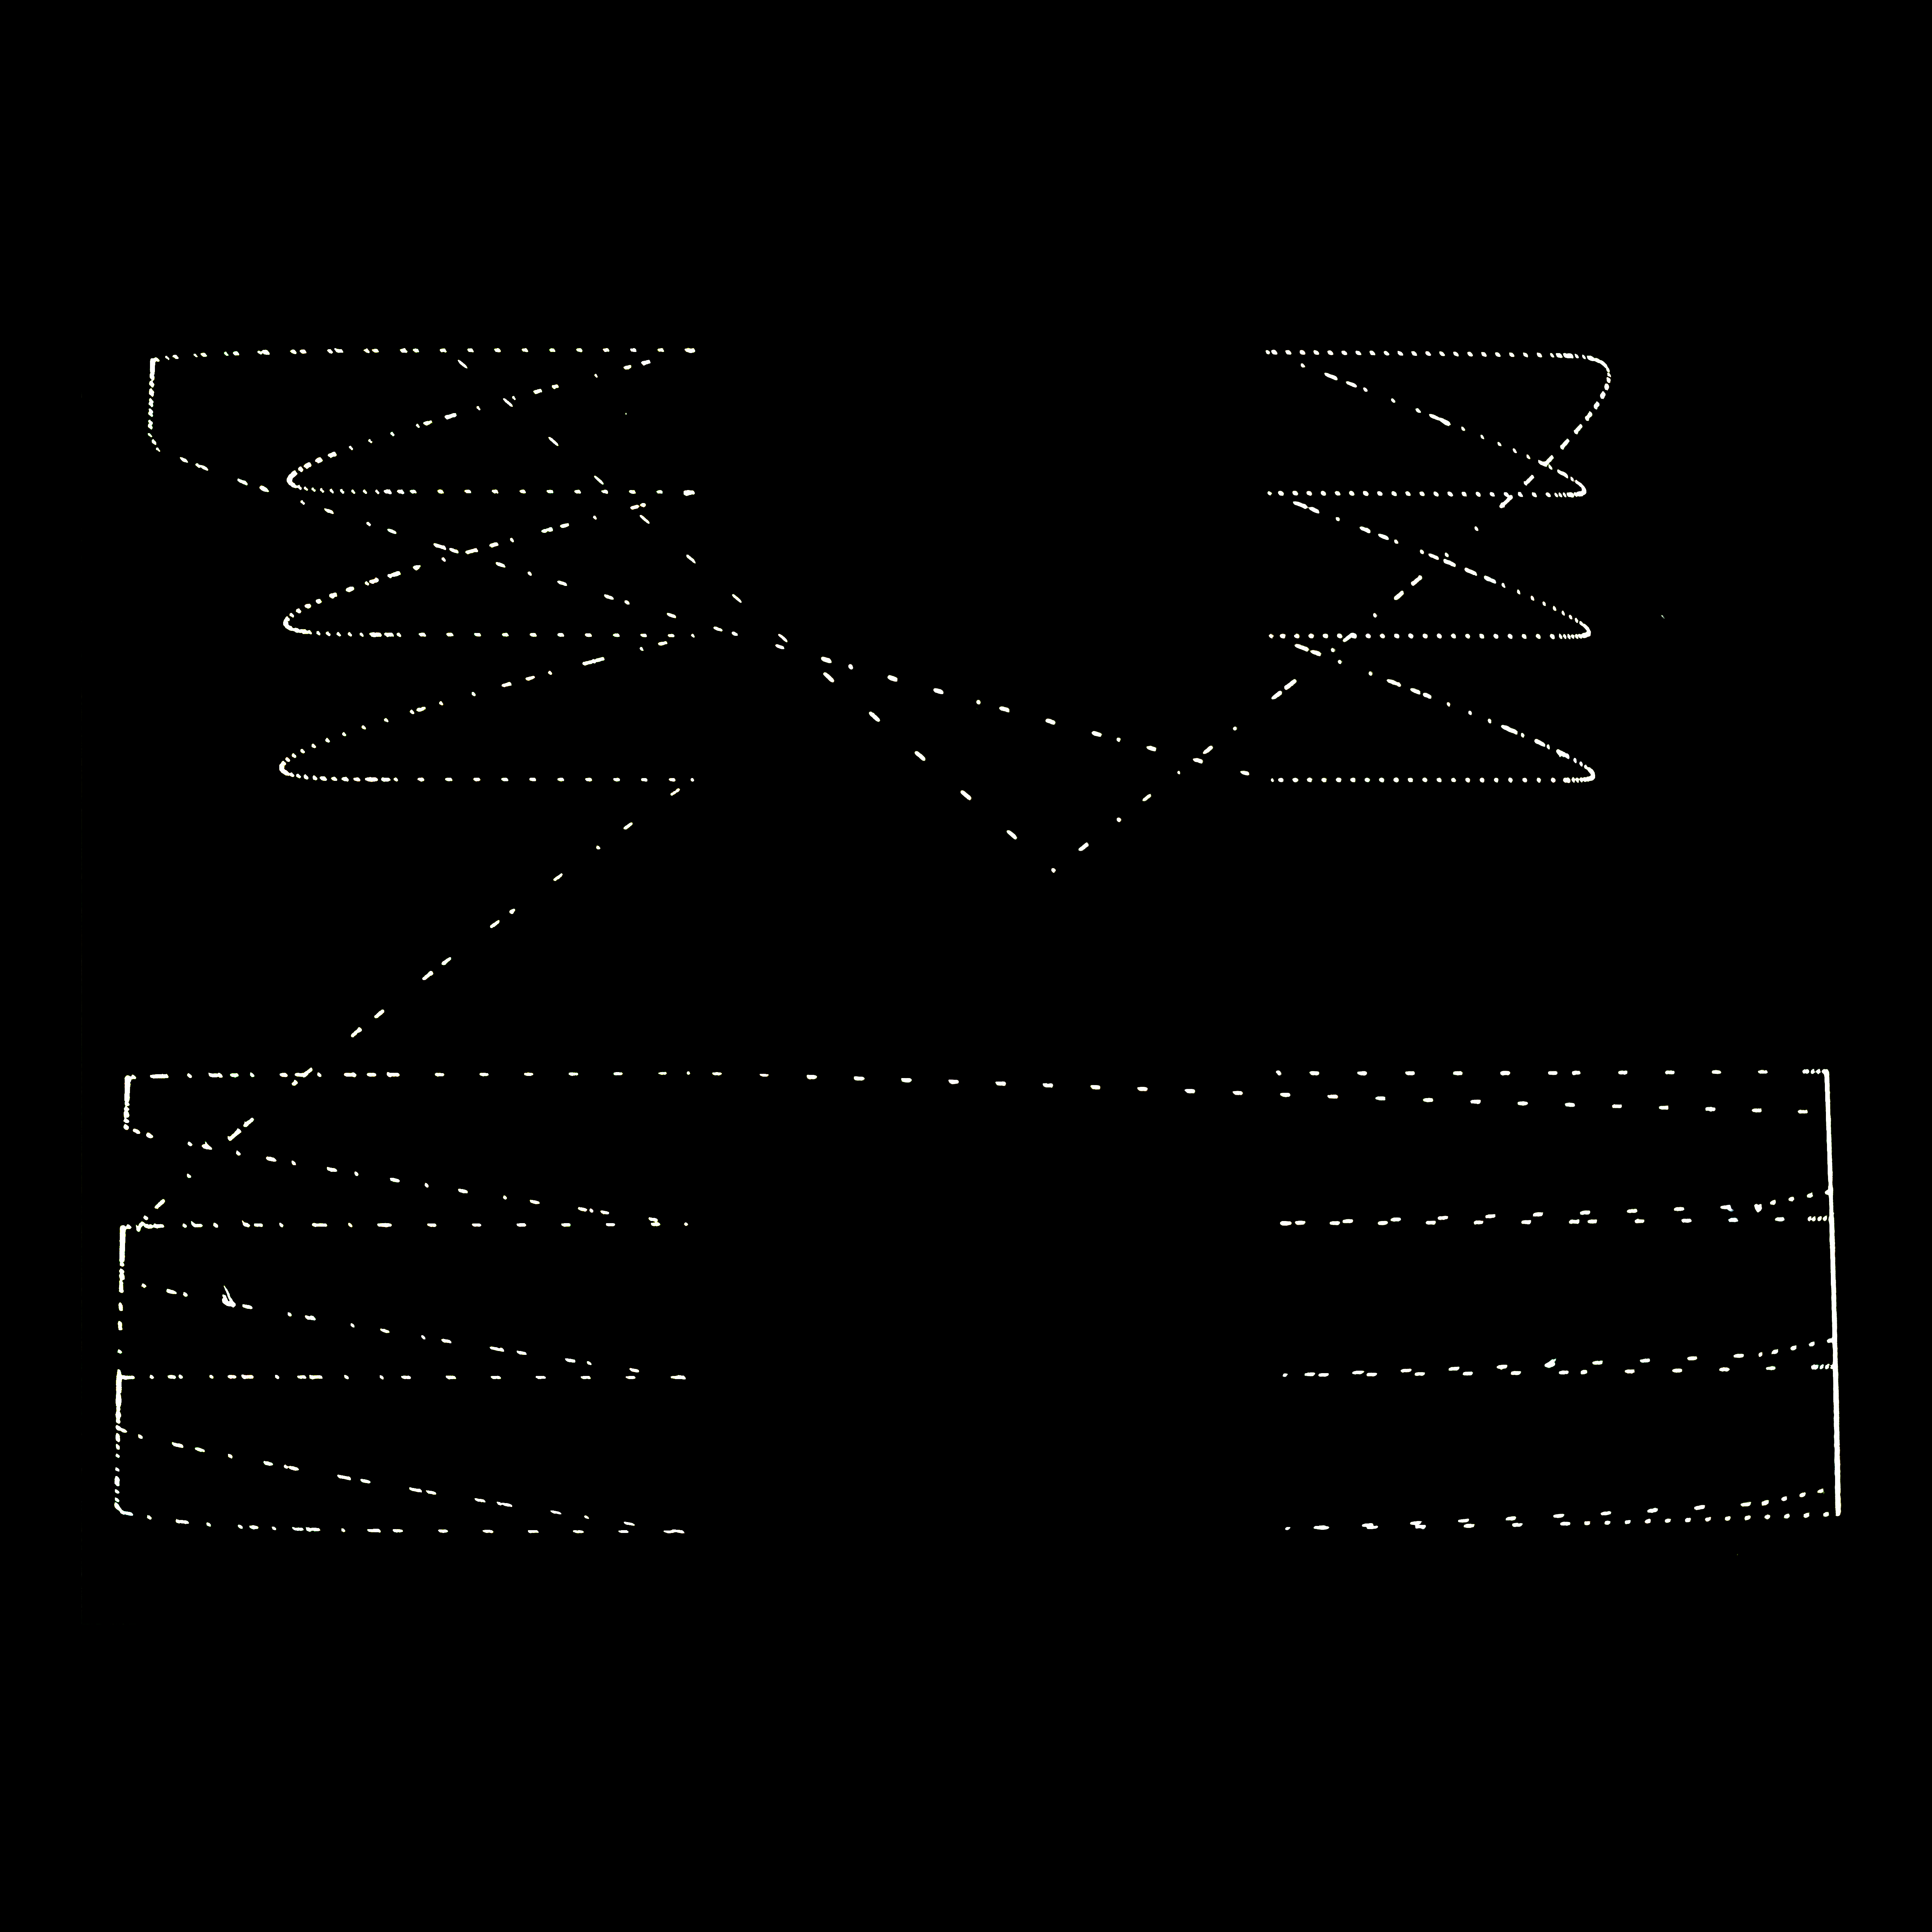
\includegraphics[width=\linewidth]{Pictures/3rd-order-high-contrast.png}
    \caption{A series of scan paths and their modified 3rd-order connecting travel trajectories traced with a pulsed laser. The line going from the centre straight in the upper left direction should be disregarded. It is a result of the laser being wrongly positioned before start, but has no influence on the rest of the experiment.}
    \label{fig:3rd-order-high-contrast}
\end{figure}

Several features can be noted from these figures. Firstly, it can be seen that the calculations in the trajectory planning seem to have been correct. The curved trajectories connect with the vertical scan trajectories at the right positions and the frequency of dots makes a smooth transition from the travel trajectory to the scan trajectory, indicating that the boundary condition on velocity has been met. The boundary conditions on acceleration are harder to verify, but at least there are no obvious indications that they should not have been met.

Also the position limit seems to have worked well with no laser lines exceeding the build plate and the curves being visibly cut-off in the bottom left and right corners.

The main difference between the quintic and cubic trajectories can be seen where the laser finishes a scan path, and starts the travel trajectory. Here the quintic trajectories have a smooth transition, ensured by the boundary conditions on velocity and acceleration. The cubic trajectories on the other hand have sharp bends and jumps in velocity because the velocity (and therefore direction) and acceleration are allowed to change instantaneously. Another difference is that the cubic polynomials overshoot the position limit more, which probably can be accredited to the fact that they are designed to start at the maximum velocity, which generally makes the paths longer.

The small dots here and there on the trace are due to the GLAMS algorithm, which at the time was made to stop the mirrors completely in between line segments. It must be admitted that this of course negated the effect of planning the smooth trajectories, but the trajectories themselves are still shown to be correct.